% Options for packages loaded elsewhere
\PassOptionsToPackage{unicode}{hyperref}
\PassOptionsToPackage{hyphens}{url}
%
\documentclass[
]{article}
\usepackage{amsmath,amssymb}
\usepackage{iftex}
\ifPDFTeX
  \usepackage[T1]{fontenc}
  \usepackage[utf8]{inputenc}
  \usepackage{textcomp} % provide euro and other symbols
\else % if luatex or xetex
  \usepackage{unicode-math} % this also loads fontspec
  \defaultfontfeatures{Scale=MatchLowercase}
  \defaultfontfeatures[\rmfamily]{Ligatures=TeX,Scale=1}
\fi
\usepackage{lmodern}
\ifPDFTeX\else
  % xetex/luatex font selection
\fi
% Use upquote if available, for straight quotes in verbatim environments
\IfFileExists{upquote.sty}{\usepackage{upquote}}{}
\IfFileExists{microtype.sty}{% use microtype if available
  \usepackage[]{microtype}
  \UseMicrotypeSet[protrusion]{basicmath} % disable protrusion for tt fonts
}{}
\makeatletter
\@ifundefined{KOMAClassName}{% if non-KOMA class
  \IfFileExists{parskip.sty}{%
    \usepackage{parskip}
  }{% else
    \setlength{\parindent}{0pt}
    \setlength{\parskip}{6pt plus 2pt minus 1pt}}
}{% if KOMA class
  \KOMAoptions{parskip=half}}
\makeatother
\usepackage{xcolor}
\usepackage[margin=1in]{geometry}
\usepackage{color}
\usepackage{fancyvrb}
\newcommand{\VerbBar}{|}
\newcommand{\VERB}{\Verb[commandchars=\\\{\}]}
\DefineVerbatimEnvironment{Highlighting}{Verbatim}{commandchars=\\\{\}}
% Add ',fontsize=\small' for more characters per line
\usepackage{framed}
\definecolor{shadecolor}{RGB}{248,248,248}
\newenvironment{Shaded}{\begin{snugshade}}{\end{snugshade}}
\newcommand{\AlertTok}[1]{\textcolor[rgb]{0.94,0.16,0.16}{#1}}
\newcommand{\AnnotationTok}[1]{\textcolor[rgb]{0.56,0.35,0.01}{\textbf{\textit{#1}}}}
\newcommand{\AttributeTok}[1]{\textcolor[rgb]{0.13,0.29,0.53}{#1}}
\newcommand{\BaseNTok}[1]{\textcolor[rgb]{0.00,0.00,0.81}{#1}}
\newcommand{\BuiltInTok}[1]{#1}
\newcommand{\CharTok}[1]{\textcolor[rgb]{0.31,0.60,0.02}{#1}}
\newcommand{\CommentTok}[1]{\textcolor[rgb]{0.56,0.35,0.01}{\textit{#1}}}
\newcommand{\CommentVarTok}[1]{\textcolor[rgb]{0.56,0.35,0.01}{\textbf{\textit{#1}}}}
\newcommand{\ConstantTok}[1]{\textcolor[rgb]{0.56,0.35,0.01}{#1}}
\newcommand{\ControlFlowTok}[1]{\textcolor[rgb]{0.13,0.29,0.53}{\textbf{#1}}}
\newcommand{\DataTypeTok}[1]{\textcolor[rgb]{0.13,0.29,0.53}{#1}}
\newcommand{\DecValTok}[1]{\textcolor[rgb]{0.00,0.00,0.81}{#1}}
\newcommand{\DocumentationTok}[1]{\textcolor[rgb]{0.56,0.35,0.01}{\textbf{\textit{#1}}}}
\newcommand{\ErrorTok}[1]{\textcolor[rgb]{0.64,0.00,0.00}{\textbf{#1}}}
\newcommand{\ExtensionTok}[1]{#1}
\newcommand{\FloatTok}[1]{\textcolor[rgb]{0.00,0.00,0.81}{#1}}
\newcommand{\FunctionTok}[1]{\textcolor[rgb]{0.13,0.29,0.53}{\textbf{#1}}}
\newcommand{\ImportTok}[1]{#1}
\newcommand{\InformationTok}[1]{\textcolor[rgb]{0.56,0.35,0.01}{\textbf{\textit{#1}}}}
\newcommand{\KeywordTok}[1]{\textcolor[rgb]{0.13,0.29,0.53}{\textbf{#1}}}
\newcommand{\NormalTok}[1]{#1}
\newcommand{\OperatorTok}[1]{\textcolor[rgb]{0.81,0.36,0.00}{\textbf{#1}}}
\newcommand{\OtherTok}[1]{\textcolor[rgb]{0.56,0.35,0.01}{#1}}
\newcommand{\PreprocessorTok}[1]{\textcolor[rgb]{0.56,0.35,0.01}{\textit{#1}}}
\newcommand{\RegionMarkerTok}[1]{#1}
\newcommand{\SpecialCharTok}[1]{\textcolor[rgb]{0.81,0.36,0.00}{\textbf{#1}}}
\newcommand{\SpecialStringTok}[1]{\textcolor[rgb]{0.31,0.60,0.02}{#1}}
\newcommand{\StringTok}[1]{\textcolor[rgb]{0.31,0.60,0.02}{#1}}
\newcommand{\VariableTok}[1]{\textcolor[rgb]{0.00,0.00,0.00}{#1}}
\newcommand{\VerbatimStringTok}[1]{\textcolor[rgb]{0.31,0.60,0.02}{#1}}
\newcommand{\WarningTok}[1]{\textcolor[rgb]{0.56,0.35,0.01}{\textbf{\textit{#1}}}}
\usepackage{longtable,booktabs,array}
\usepackage{calc} % for calculating minipage widths
% Correct order of tables after \paragraph or \subparagraph
\usepackage{etoolbox}
\makeatletter
\patchcmd\longtable{\par}{\if@noskipsec\mbox{}\fi\par}{}{}
\makeatother
% Allow footnotes in longtable head/foot
\IfFileExists{footnotehyper.sty}{\usepackage{footnotehyper}}{\usepackage{footnote}}
\makesavenoteenv{longtable}
\usepackage{graphicx}
\makeatletter
\def\maxwidth{\ifdim\Gin@nat@width>\linewidth\linewidth\else\Gin@nat@width\fi}
\def\maxheight{\ifdim\Gin@nat@height>\textheight\textheight\else\Gin@nat@height\fi}
\makeatother
% Scale images if necessary, so that they will not overflow the page
% margins by default, and it is still possible to overwrite the defaults
% using explicit options in \includegraphics[width, height, ...]{}
\setkeys{Gin}{width=\maxwidth,height=\maxheight,keepaspectratio}
% Set default figure placement to htbp
\makeatletter
\def\fps@figure{htbp}
\makeatother
\setlength{\emergencystretch}{3em} % prevent overfull lines
\providecommand{\tightlist}{%
  \setlength{\itemsep}{0pt}\setlength{\parskip}{0pt}}
\setcounter{secnumdepth}{-\maxdimen} % remove section numbering
\ifLuaTeX
  \usepackage{selnolig}  % disable illegal ligatures
\fi
\usepackage{bookmark}
\IfFileExists{xurl.sty}{\usepackage{xurl}}{} % add URL line breaks if available
\urlstyle{same}
\hypersetup{
  pdftitle={Projet Machine Learning},
  pdfauthor={Fatima HADDAG, Cylia OUABA, Yikun WANG, Imane ALLAOUI},
  hidelinks,
  pdfcreator={LaTeX via pandoc}}

\title{Projet Machine Learning}
\author{Fatima HADDAG, Cylia OUABA, Yikun WANG, Imane ALLAOUI}
\date{2025-01-10}

\begin{document}
\maketitle

\section{Introduction}\label{introduction}

Les catastrophes naturelles constituent l'un des défis majeurs de notre
époque, avec des impacts dévastateurs sur les populations et les
économies mondiales. Face à ces enjeux, la capacité à prédire et à
évaluer leurs conséquences devient cruciale, particulièrement pour le
secteur de l'assurance qui joue un rôle central dans la gestion des
risques.

Ce projet s'appuie sur la base de données \textbf{EM-DAT} (Emergency
Events Database), qui recense les catastrophes naturelles survenues à
l'échelle mondiale entre 1980 et 2024. Cette base de données fournit des
informations détaillées sur :

\begin{itemize}
\item
  Les types de catastrophes (inondations, séismes, épidémies\ldots)
\item
  Leur localisation géographique
\item
  Leurs impacts humains (décès, personnes affectées)
\end{itemize}

Notre étude vise à répondre à la problématique suivante :

\textbf{Comment prévoir l'impact humain des catastrophes naturelles en
termes de décès et de populations affectées, et utiliser ces prévisions
pour proposer une solution concrète aux assureurs ?}

Les objectifs spécifiques sont :

\begin{enumerate}
\def\labelenumi{\arabic{enumi}.}
\tightlist
\item
  \textbf{Prédire l'impact des catastrophes} :

  \begin{itemize}
  \tightlist
  \item
    Estimer le nombre de décès
  \item
    Évaluer le nombre de personnes affectées (blessés, déplacés,
    nécessitant une assistance)
  \item
    Analyser les facteurs déterminants de ces impacts
  \end{itemize}
\item
  \textbf{Proposer une méthodologie pour le secteur de l'assurance} :

  \begin{itemize}
  \tightlist
  \item
    Développer un modèle prédictif fiable
  \item
    Fournir des outils d'aide à la décision pour la tarification
  \item
    Améliorer l'évaluation des risques
  \end{itemize}
\end{enumerate}

Cette approche combinera des analyses statistiques avancées et des
techniques de machine learning pour développer des modèles prédictifs
robustes et applicables dans un contexte professionnel.

\section{1. Traitement et analyse des
données}\label{traitement-et-analyse-des-donnuxe9es}

\subsection{1.1 Importation et aperçu des
données}\label{importation-et-aperuxe7u-des-donnuxe9es}

\begin{verbatim}
## Rows: 14,936
## Columns: 15
## $ disaster_subgroup <chr> "Geophysical", "Biological", "Hydrological", "Biolog~
## $ disaster_type     <chr> "Earthquake", "Epidemic", "Flood", "Epidemic", "Floo~
## $ disaster_subtype  <chr> "Ground movement", "Bacterial disease", "Flood (Gene~
## $ iso_code          <chr> "AZO", "MUS", "BOL", "LBR", "BRA", "PHL", "IND", "RE~
## $ country           <chr> "Azores Islands", "Mauritius", "Bolivia (Plurination~
## $ subregion         <chr> "Southern Europe", "Sub-Saharan Africa", "Latin Amer~
## $ region            <chr> "Europe", "Africa", "Americas", "Africa", "Americas"~
## $ location          <chr> "Terceira, San Miguel, Santa Maria Pico, Sao Jorge I~
## $ magnitude_scale   <chr> "Moment Magnitude", "Non applicable", "Km2", "Non ap~
## $ total_deaths      <dbl> 69, NA, NA, 466, 17, 2, 79, 25, 50, 6, NA, 75, 10, 1~
## $ total_affected    <dbl> 21900, 108, 15000, 1887, 1000, 25980, NA, 7000, 2700~
## $ year              <dbl> 1980, 1980, 1980, 1980, 1980, 1980, 1980, 1980, 1980~
## $ start_date        <date> 1980-01-01, 1980-01-01, NA, 1980-01-01, NA, NA, NA,~
## $ end_date          <date> 1980-01-01, 1980-01-01, NA, 1980-01-01, NA, NA, NA,~
## $ event_duration    <dbl> 0, 0, NA, 0, NA, NA, NA, 0, NA, NA, NA, NA, 0, 0, NA~
\end{verbatim}

\subsection{1.2 Analyse des valeurs
manquantes}\label{analyse-des-valeurs-manquantes}

\begin{longtable}[]{@{}llr@{}}
\caption{Pourcentage de valeurs manquantes par variable}\tabularnewline
\toprule\noalign{}
& Variable & Missing\_Percentage \\
\midrule\noalign{}
\endfirsthead
\toprule\noalign{}
& Variable & Missing\_Percentage \\
\midrule\noalign{}
\endhead
\bottomrule\noalign{}
\endlastfoot
disaster\_subgroup & disaster\_subgroup & 0 \\
disaster\_type & disaster\_type & 0 \\
disaster\_subtype & disaster\_subtype & 0 \\
iso\_code & iso\_code & 0 \\
country & country & 0 \\
subregion & subregion & 0 \\
region & region & 0 \\
location & location & 0 \\
magnitude\_scale & magnitude\_scale & 0 \\
total\_deaths & total\_deaths & 30 \\
total\_affected & total\_affected & 23 \\
year & year & 0 \\
start\_date & start\_date & 19 \\
end\_date & end\_date & 18 \\
event\_duration & event\_duration & 20 \\
\end{longtable}

Cette première analyse nous permet d'observer :

\begin{enumerate}
\def\labelenumi{\arabic{enumi}.}
\item
  La structure de notre jeu de données avec ses différentes variables
\item
  La présence et la distribution des valeurs manquantes
\item
  La qualité générale des données
\end{enumerate}

L'analyse préliminaire des valeurs manquantes révèle que certaines
variables clés comme \texttt{total\_deaths} et \texttt{total\_affected}
présentent respectivement 30\% et 23\% de valeurs manquantes. Ces
proportions significatives nécessitent une étude plus approfondie des
patterns de données manquantes selon différentes dimensions (région,
type de catastrophe, période) pour guider notre stratégie de traitement
des données.

Procédons à une analyse plus détaillée de ces valeurs manquantes :

\subsection{1.3 Analyse détaillée des valeurs
manquantes}\label{analyse-duxe9tailluxe9e-des-valeurs-manquantes}

\subsubsection{1.3.1 Analyse par dimension (région, type et
temporelle)}\label{analyse-par-dimension-ruxe9gion-type-et-temporelle}

\subsubsection{1.3.2 Visualisation des patterns de valeurs
manquantes}\label{visualisation-des-patterns-de-valeurs-manquantes}

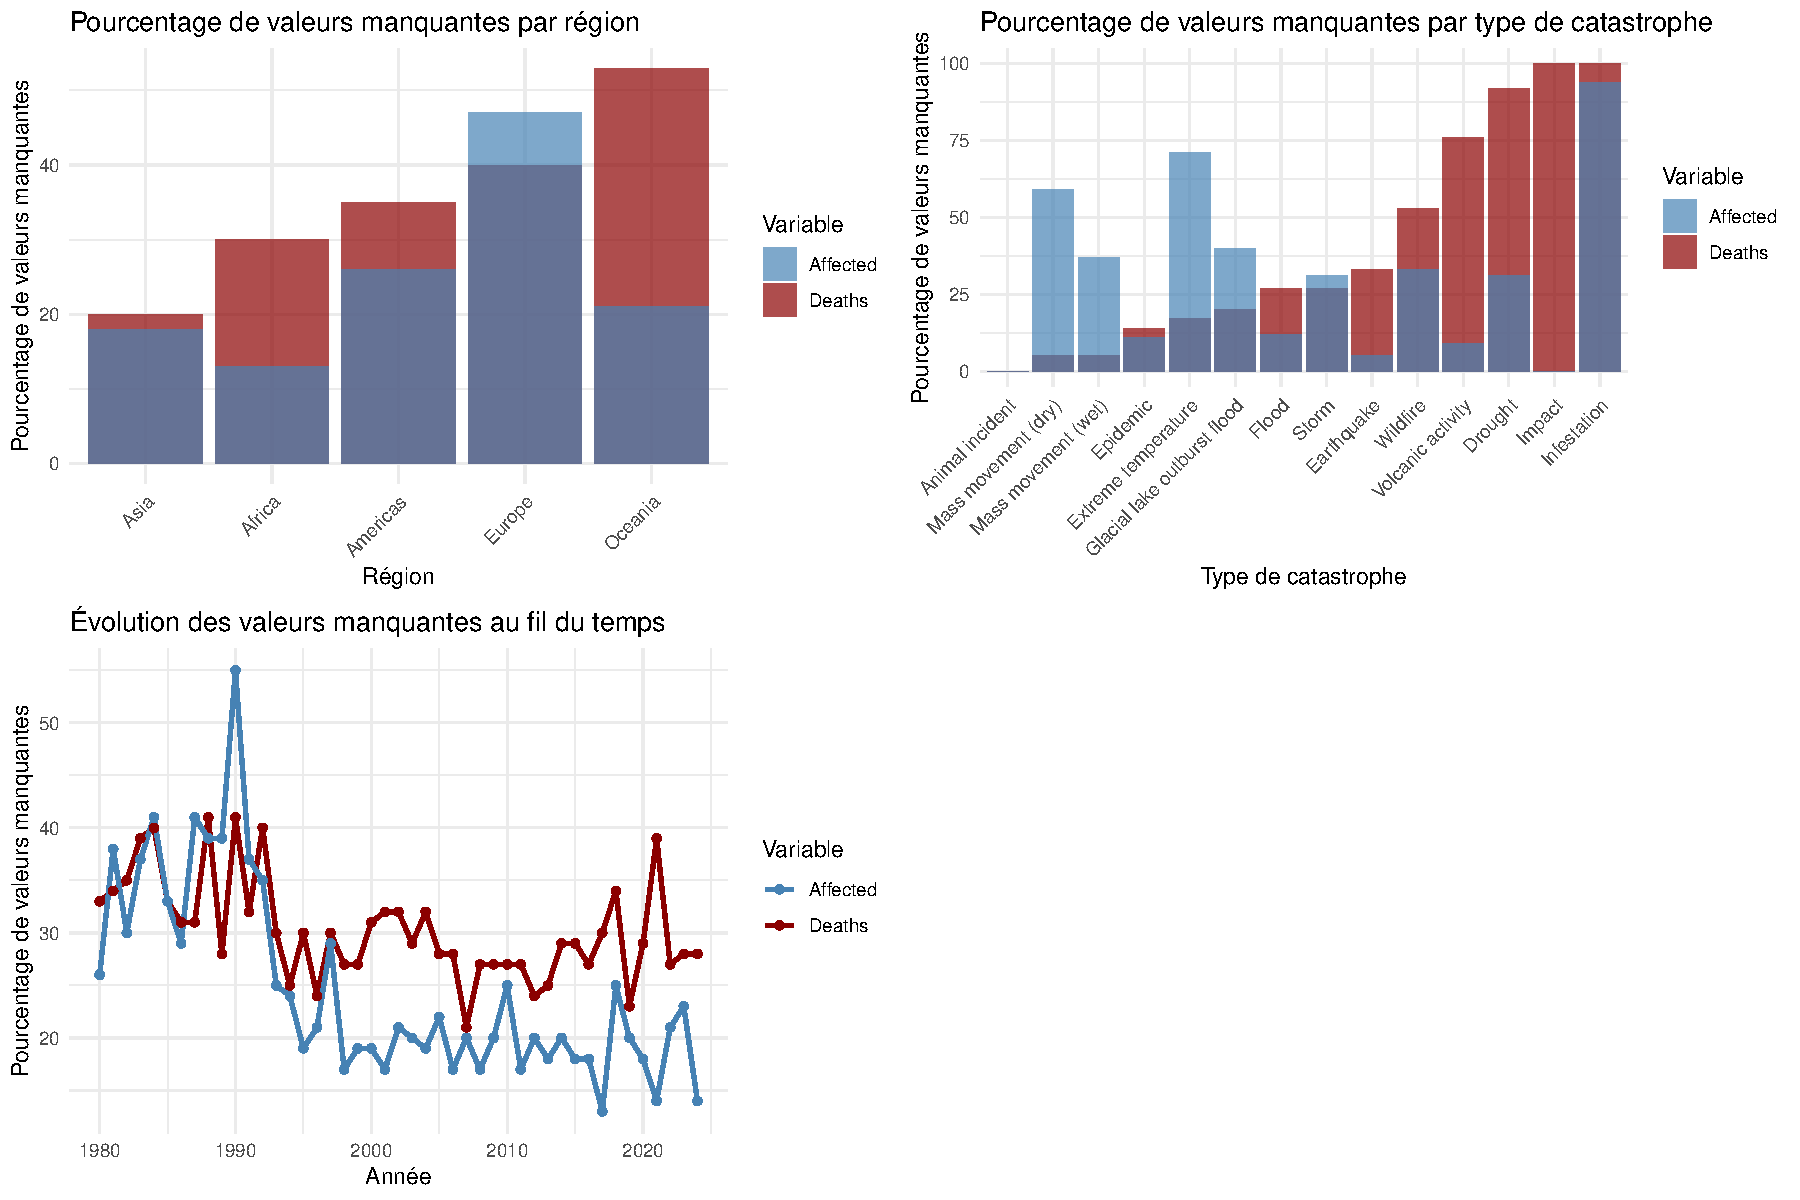
\includegraphics{Projet_ML_files/figure-latex/missing_plots-1.pdf}

Cette analyse visuelle des valeurs manquantes révèle plusieurs patterns
importants :

\begin{enumerate}
\def\labelenumi{\arabic{enumi}.}
\tightlist
\item
  \textbf{Distribution géographique} :

  \begin{itemize}
  \tightlist
  \item
    L'Océanie et l'Europe présentent les plus hauts taux de valeurs
    manquantes
  \item
    L'Asie montre le taux le plus faible, suggérant une meilleure
    qualité de collecte des données
  \end{itemize}
\item
  \textbf{Par type de catastrophe} :

  \begin{itemize}
  \tightlist
  \item
    Certains types comme ``Impact'' et ``Infestation'' ont des taux très
    élevés de données manquantes
  \item
    Les catastrophes de type ``Mass movement'' et ``Animal incident''
    sont mieux documentées
  \end{itemize}
\item
  \textbf{Évolution temporelle} :

  \begin{itemize}
  \tightlist
  \item
    Une tendance à la stabilisation des taux de valeurs manquantes
    depuis les années 2000
  \item
    Une amélioration générale de la collecte de données par rapport aux
    années 1980-1990
  \end{itemize}
\end{enumerate}

Ces observations vont nous guider dans notre stratégie de traitement des
données manquantes.

\subsection{1.4 Traitement des valeurs
manquantes}\label{traitement-des-valeurs-manquantes}

Face à ces patterns de valeurs manquantes, nous optons pour une approche
de suppression simple des observations incomplètes pour garantir la
fiabilité de nos analyses futures.

\begin{verbatim}
## Dimensions avant nettoyage : 14936 15
\end{verbatim}

\begin{verbatim}
## Dimensions après nettoyage : 7148 15
\end{verbatim}

\begin{verbatim}
## Pourcentage de données conservées : 47.86 %
\end{verbatim}

\begin{longtable}[]{@{}lrr@{}}
\caption{Comparaison des statistiques avant et après
nettoyage}\tabularnewline
\toprule\noalign{}
Statistique & Avant & Après \\
\midrule\noalign{}
\endfirsthead
\toprule\noalign{}
Statistique & Avant & Après \\
\midrule\noalign{}
\endhead
\bottomrule\noalign{}
\endlastfoot
Nombre d'observations & 14936.0 & 7148.00 \\
Moyenne des décès & 278.7 & 250.81 \\
Médiane des décès & 15.0 & 13.00 \\
Moyenne des affectés & 693686.2 & 631806.86 \\
Médiane des affectés & 5788.0 & 6900.00 \\
\end{longtable}

Notre processus de nettoyage a conduit à une réduction significative du
jeu de données, passant de 14,936 à 7,148 observations (47.86\% des
données initiales conservées). Malgré cette réduction importante,
plusieurs éléments justifient notre choix :

\begin{enumerate}
\def\labelenumi{\arabic{enumi}.}
\item
  \textbf{Volume suffisant} : Plus de 7,000 observations restent
  disponibles pour l'analyse et la modélisation
\item
  \textbf{Qualité des données} : Les statistiques descriptives
  avant/après nettoyage montrent que la structure générale des données
  est préservée
\item
  \textbf{Fiabilité} : Les observations conservées sont complètes et
  permettront des analyses robustes
\end{enumerate}

À présent que nos données sont nettoyées, nous pouvons procéder à leur
analyse descriptive détaillée.

\section{2. Analyse Exploratoire des
Données}\label{analyse-exploratoire-des-donnuxe9es}

\subsection{2.1 Analyse Descriptive
Univariée}\label{analyse-descriptive-univariuxe9e}

Notre objectif étant de prédire l'impact humain des catastrophes
naturelles, nous nous concentrons sur la variable \texttt{total\_deaths}
comme variable d'intérêt principale. Cette variable représente le nombre
total de décès directement attribuables à chaque catastrophe naturelle,
constituant ainsi un indicateur crucial de la gravité de l'événement.

\subsubsection{2.1.1 Sélection des variables
explicatives}\label{suxe9lection-des-variables-explicatives}

Pour prédire le nombre de décès, nous avons identifié plusieurs
variables explicatives pertinentes :

\begin{longtable}[]{@{}
  >{\raggedright\arraybackslash}p{(\columnwidth - 2\tabcolsep) * \real{0.1771}}
  >{\raggedright\arraybackslash}p{(\columnwidth - 2\tabcolsep) * \real{0.8229}}@{}}
\caption{Variables explicatives sélectionnées et leur
justification}\tabularnewline
\toprule\noalign{}
\begin{minipage}[b]{\linewidth}\raggedright
Variable
\end{minipage} & \begin{minipage}[b]{\linewidth}\raggedright
Justification
\end{minipage} \\
\midrule\noalign{}
\endfirsthead
\toprule\noalign{}
\begin{minipage}[b]{\linewidth}\raggedright
Variable
\end{minipage} & \begin{minipage}[b]{\linewidth}\raggedright
Justification
\end{minipage} \\
\midrule\noalign{}
\endhead
\bottomrule\noalign{}
\endlastfoot
disaster\_type & Nature de la catastrophe, influençant directement le
potentiel de mortalité \\
disaster\_subtype & Précision sur le type spécifique, permettant une
granularité plus fine \\
region & Zone géographique, reflétant les différences de vulnérabilité
et de résilience \\
total\_affected & Ampleur de l'impact sur la population, fortement
corrélée aux décès \\
event\_duration & Durée de l'événement, pouvant influencer la gravité
des impacts \\
year & Année de l'événement, capturant l'évolution des capacités de
réponse \\
\end{longtable}

\subsubsection{2.1.2 Distribution de la variable d'intérêt : Total
Deaths}\label{distribution-de-la-variable-dintuxe9ruxeat-total-deaths}

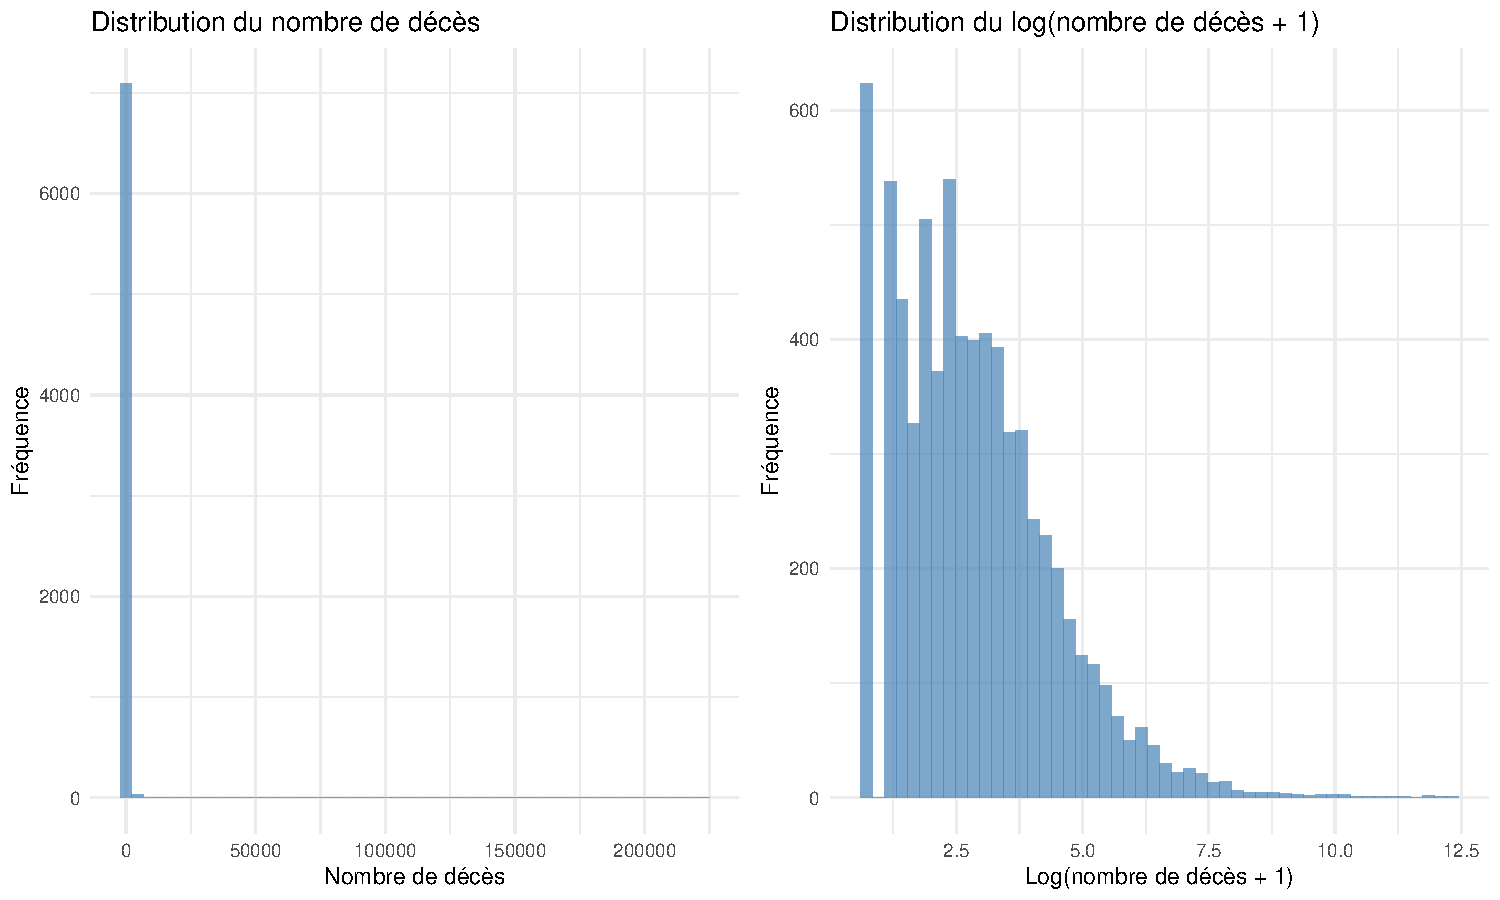
\includegraphics{Projet_ML_files/figure-latex/distribution_target-1.pdf}

\begin{longtable}[]{@{}lrr@{}}
\caption{Statistiques descriptives du nombre de décès et de leur
logarithme}\tabularnewline
\toprule\noalign{}
Statistiques & Décès & Log\_Décès \\
\midrule\noalign{}
\endfirsthead
\toprule\noalign{}
Statistiques & Décès & Log\_Décès \\
\midrule\noalign{}
\endhead
\bottomrule\noalign{}
\endlastfoot
Minimum & 1.00 & 0.69 \\
1er Quartile & 4.00 & 1.61 \\
Médiane & 13.00 & 2.64 \\
Moyenne & 250.81 & 2.85 \\
3e Quartile & 41.00 & 3.74 \\
Maximum & 222570.00 & 12.31 \\
Écart-type & 4420.58 & 1.58 \\
\end{longtable}

La distribution de notre variable cible \texttt{total\_deaths} présente
une forte asymétrie positive, caractéristique courante des données de
catastrophes naturelles. Cette distribution justifie :

\begin{enumerate}
\def\labelenumi{\arabic{enumi}.}
\tightlist
\item
  L'utilisation d'une transformation logarithmique pour nos analyses et
  modélisations futures
\item
  La nécessité de tenir compte des valeurs extrêmes qui représentent des
  catastrophes majeures
\item
  L'importance d'une approche robuste dans notre méthodologie de
  prédiction
\end{enumerate}

L'analyse des statistiques descriptives révèle plusieurs points
importants :

\begin{enumerate}
\def\labelenumi{\arabic{enumi}.}
\tightlist
\item
  \textbf{Distribution fortement asymétrique des décès} :

  \begin{itemize}
  \tightlist
  \item
    La moyenne (250.81) est nettement supérieure à la médiane (13.00),
    indiquant une forte asymétrie à droite
  \item
    L'écart important entre la médiane et le maximum (222,570) montre la
    présence de valeurs extrêmes
  \item
    75\% des catastrophes causent moins de 41 décès (3e quartile),
    tandis que certains événements extrêmes peuvent causer plus de
    200,000 décès
  \end{itemize}
\item
  \textbf{Effet de la transformation logarithmique} :

  \begin{itemize}
  \tightlist
  \item
    La transformation log réduit considérablement l'écart entre la
    moyenne (2.85) et la médiane (2.64)
  \item
    L'écart-type passe de 4420.58 à 1.58, indiquant une stabilisation de
    la variance
  \item
    Les valeurs extrêmes sont mieux gérées : le maximum passe de 222,570
    à 12.31 sur l'échelle logarithmique
  \end{itemize}
\end{enumerate}

Cette transformation logarithmique s'avère donc pertinente pour : -
Réduire l'influence des valeurs extrêmes - Stabiliser la variance -
Obtenir une distribution plus proche de la normale, ce qui sera
bénéfique pour nos futures analyses statistiques et modélisations

\subsubsection{2.1.3 Variables
quantitatives}\label{variables-quantitatives}

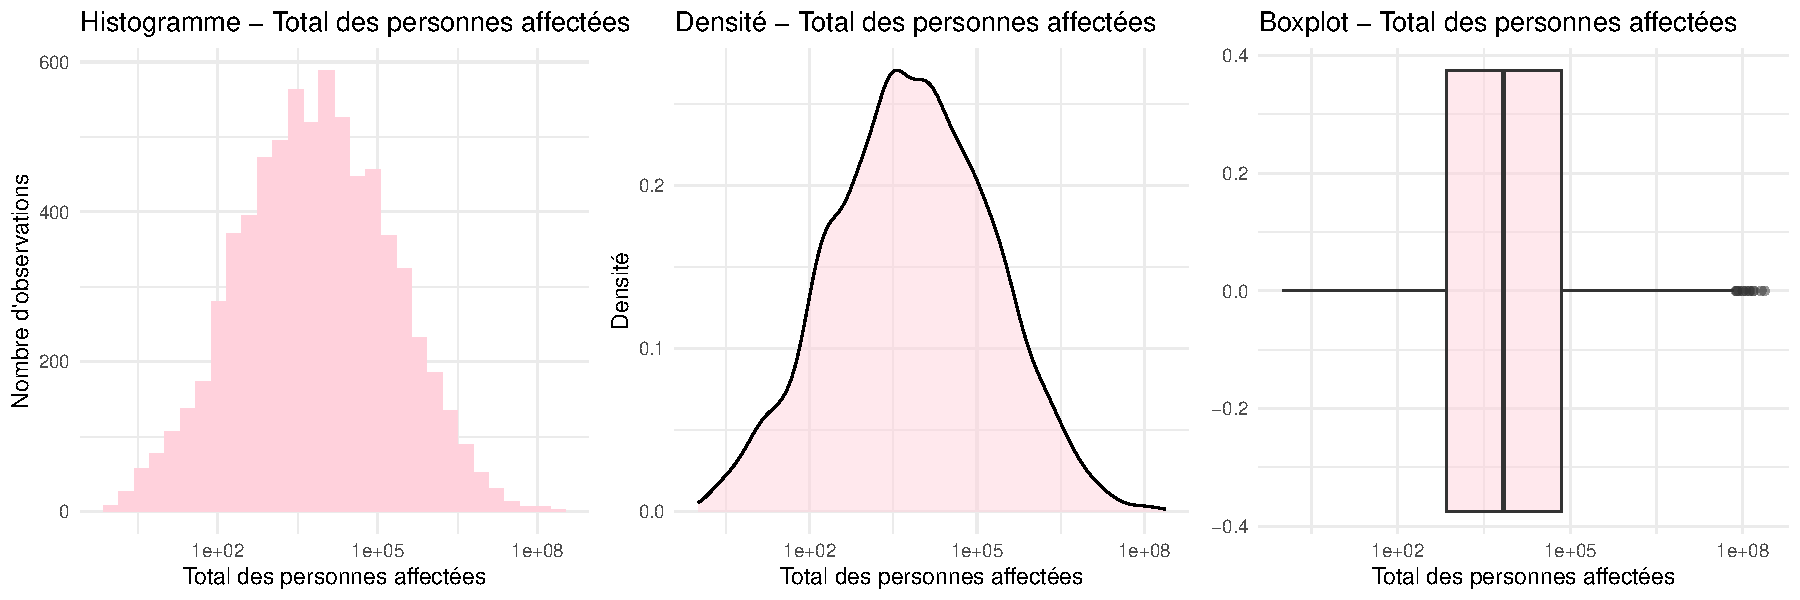
\includegraphics{Projet_ML_files/figure-latex/quantitative_vars-1.pdf}

\textbf{Interprétation pour Total Affected :} L'analyse de la
distribution des personnes affectées révèle une asymétrie forte avec la
majorité des catastrophes touchant entre 10³ et 10⁵ personnes. Les
valeurs extrêmes, représentant des catastrophes majeures affectant des
millions de personnes, sont nombreuses mais plus rares. Cette
distribution fortement asymétrique justifie l'utilisation d'une échelle
logarithmique pour nos analyses futures et suggère des impacts très
variables selon le type et l'ampleur des catastrophes.

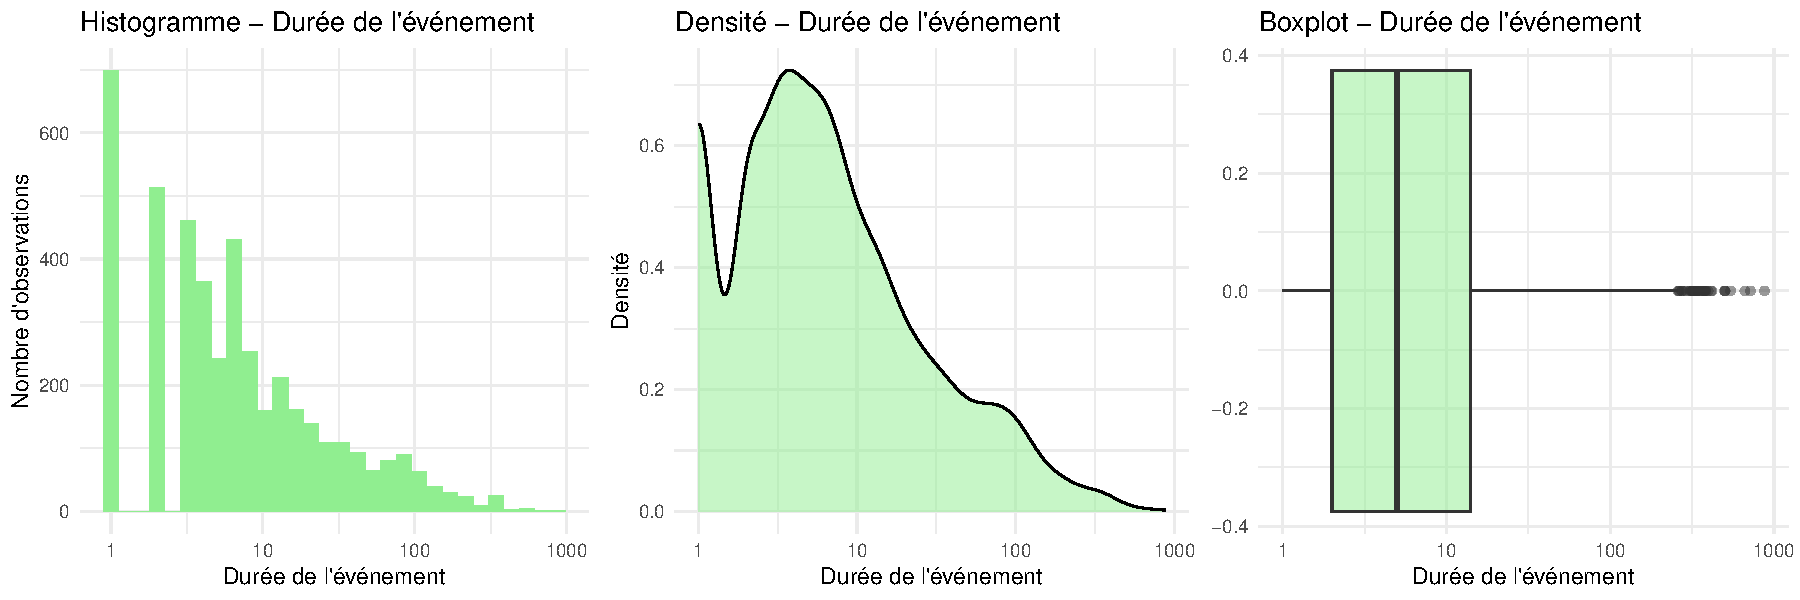
\includegraphics{Projet_ML_files/figure-latex/quantitative_vars 2-1.pdf}

\textbf{Interprétation pour Event Duration :} La durée des événements
montre également une distribution asymétrique avec une concentration
marquée sur des durées courtes (1-10 jours). Le pic initial suivi d'une
décroissance rapide indique que la plupart des catastrophes sont de
courte durée, mais certaines peuvent s'étendre sur plusieurs semaines,
voire mois (valeurs extrêmes \textgreater{} 100 jours). Cette
distribution suggère l'importance de distinguer les catastrophes
ponctuelles des événements prolongés dans nos analyses.

\subsubsection{2.1.4 Variables
qualitatives}\label{variables-qualitatives}

\begin{center}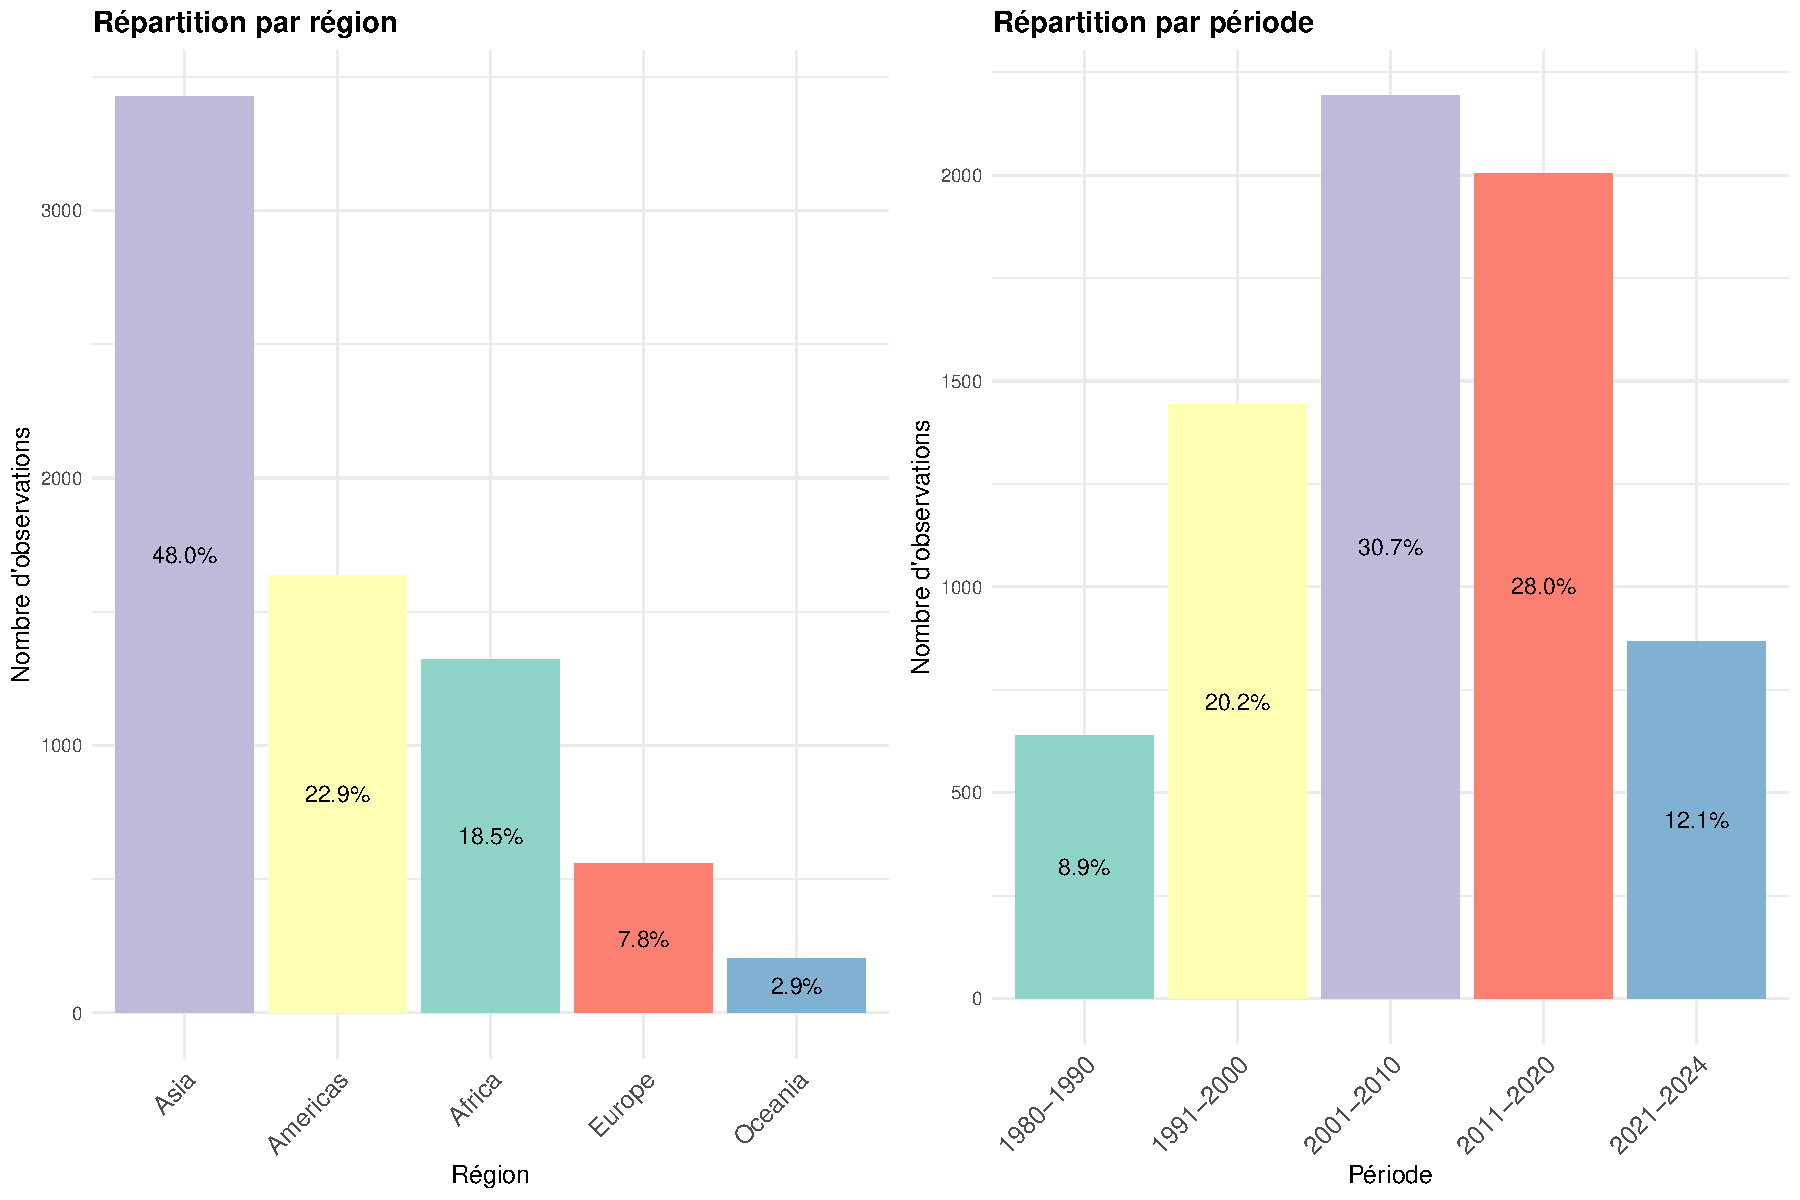
\includegraphics[width=1\linewidth]{Projet_ML_files/figure-latex/unnamed-chunk-2-1} \end{center}

\begin{center}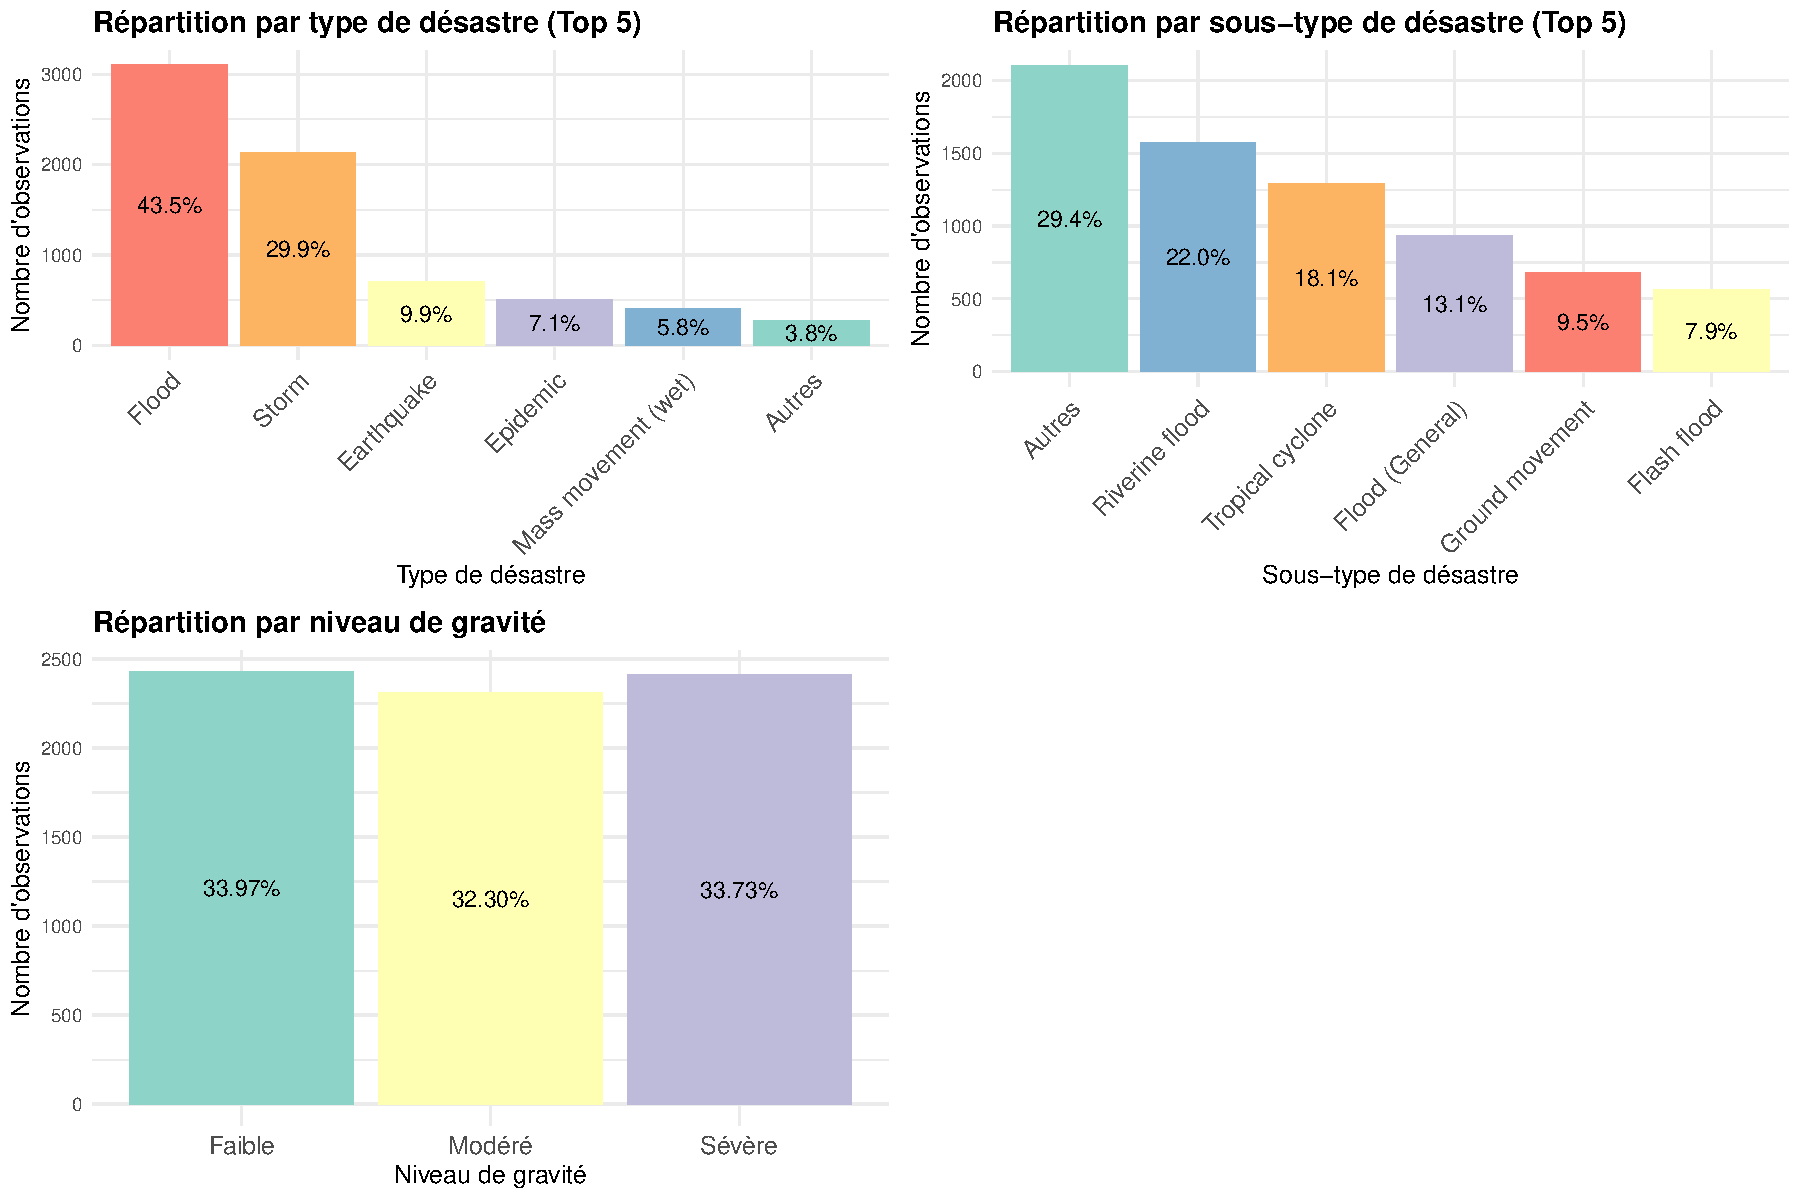
\includegraphics[width=1\linewidth]{Projet_ML_files/figure-latex/unnamed-chunk-2-2} \end{center}

L'analyse de la distribution des catastrophes naturelles révèle
plusieurs aspects importants :

\begin{enumerate}
\def\labelenumi{\arabic{enumi}.}
\tightlist
\item
  \textbf{Distribution par niveau de gravité} :
\end{enumerate}

\begin{itemize}
\tightlist
\item
  La répartition est remarquablement équilibrée entre les trois niveaux
  de gravité (environ 33\% chacun)
\item
  Cette distribution équilibrée résulte de notre catégorisation basée
  sur les terciles du logarithme du nombre de décès
\end{itemize}

\begin{enumerate}
\def\labelenumi{\arabic{enumi}.}
\setcounter{enumi}{1}
\tightlist
\item
  \textbf{Distribution par type de catastrophe} :
\end{enumerate}

\begin{itemize}
\tightlist
\item
  Les inondations (Flood) dominent largement avec 43.5\% des événements
\item
  Les tempêtes (Storm) représentent près d'un tiers des catastrophes
  (29.9\%)
\item
  Les séismes (Earthquake) constituent 9.9\% des événements
\item
  Les épidémies et les mouvements de masse sont moins fréquents
  (\textless8\% chacun)
\end{itemize}

\begin{enumerate}
\def\labelenumi{\arabic{enumi}.}
\setcounter{enumi}{2}
\tightlist
\item
  \textbf{Analyse des sous-types de catastrophes} :
\end{enumerate}

\begin{itemize}
\tightlist
\item
  Les inondations se décomposent en plusieurs sous-types :

  \begin{itemize}
  \tightlist
  \item
    Riverine flood (22.0\%)
  \item
    Flash flood (7.9\%)
  \item
    Flood General (13.1\%)
  \end{itemize}
\item
  Les cyclones tropicaux représentent 18.1\% des événements
\item
  Les mouvements de terrain (Ground movement) constituent 9.5\%
\item
  La catégorie ``Autres'' (29.4\%) regroupe de nombreux sous-types moins
  fréquents
\end{itemize}

Cette distribution détaillée souligne l'importance particulière des
inondations et de leurs différentes manifestations dans notre jeu de
données, ainsi que la grande diversité des catastrophes naturelles
étudiées.

\subsection{2.2 Analyse Bivariée}\label{analyse-bivariuxe9e}

\subsubsection{2.2.1 Distribution de la variable d'intérêt selon les
variables
catégorielles}\label{distribution-de-la-variable-dintuxe9ruxeat-selon-les-variables-catuxe9gorielles}

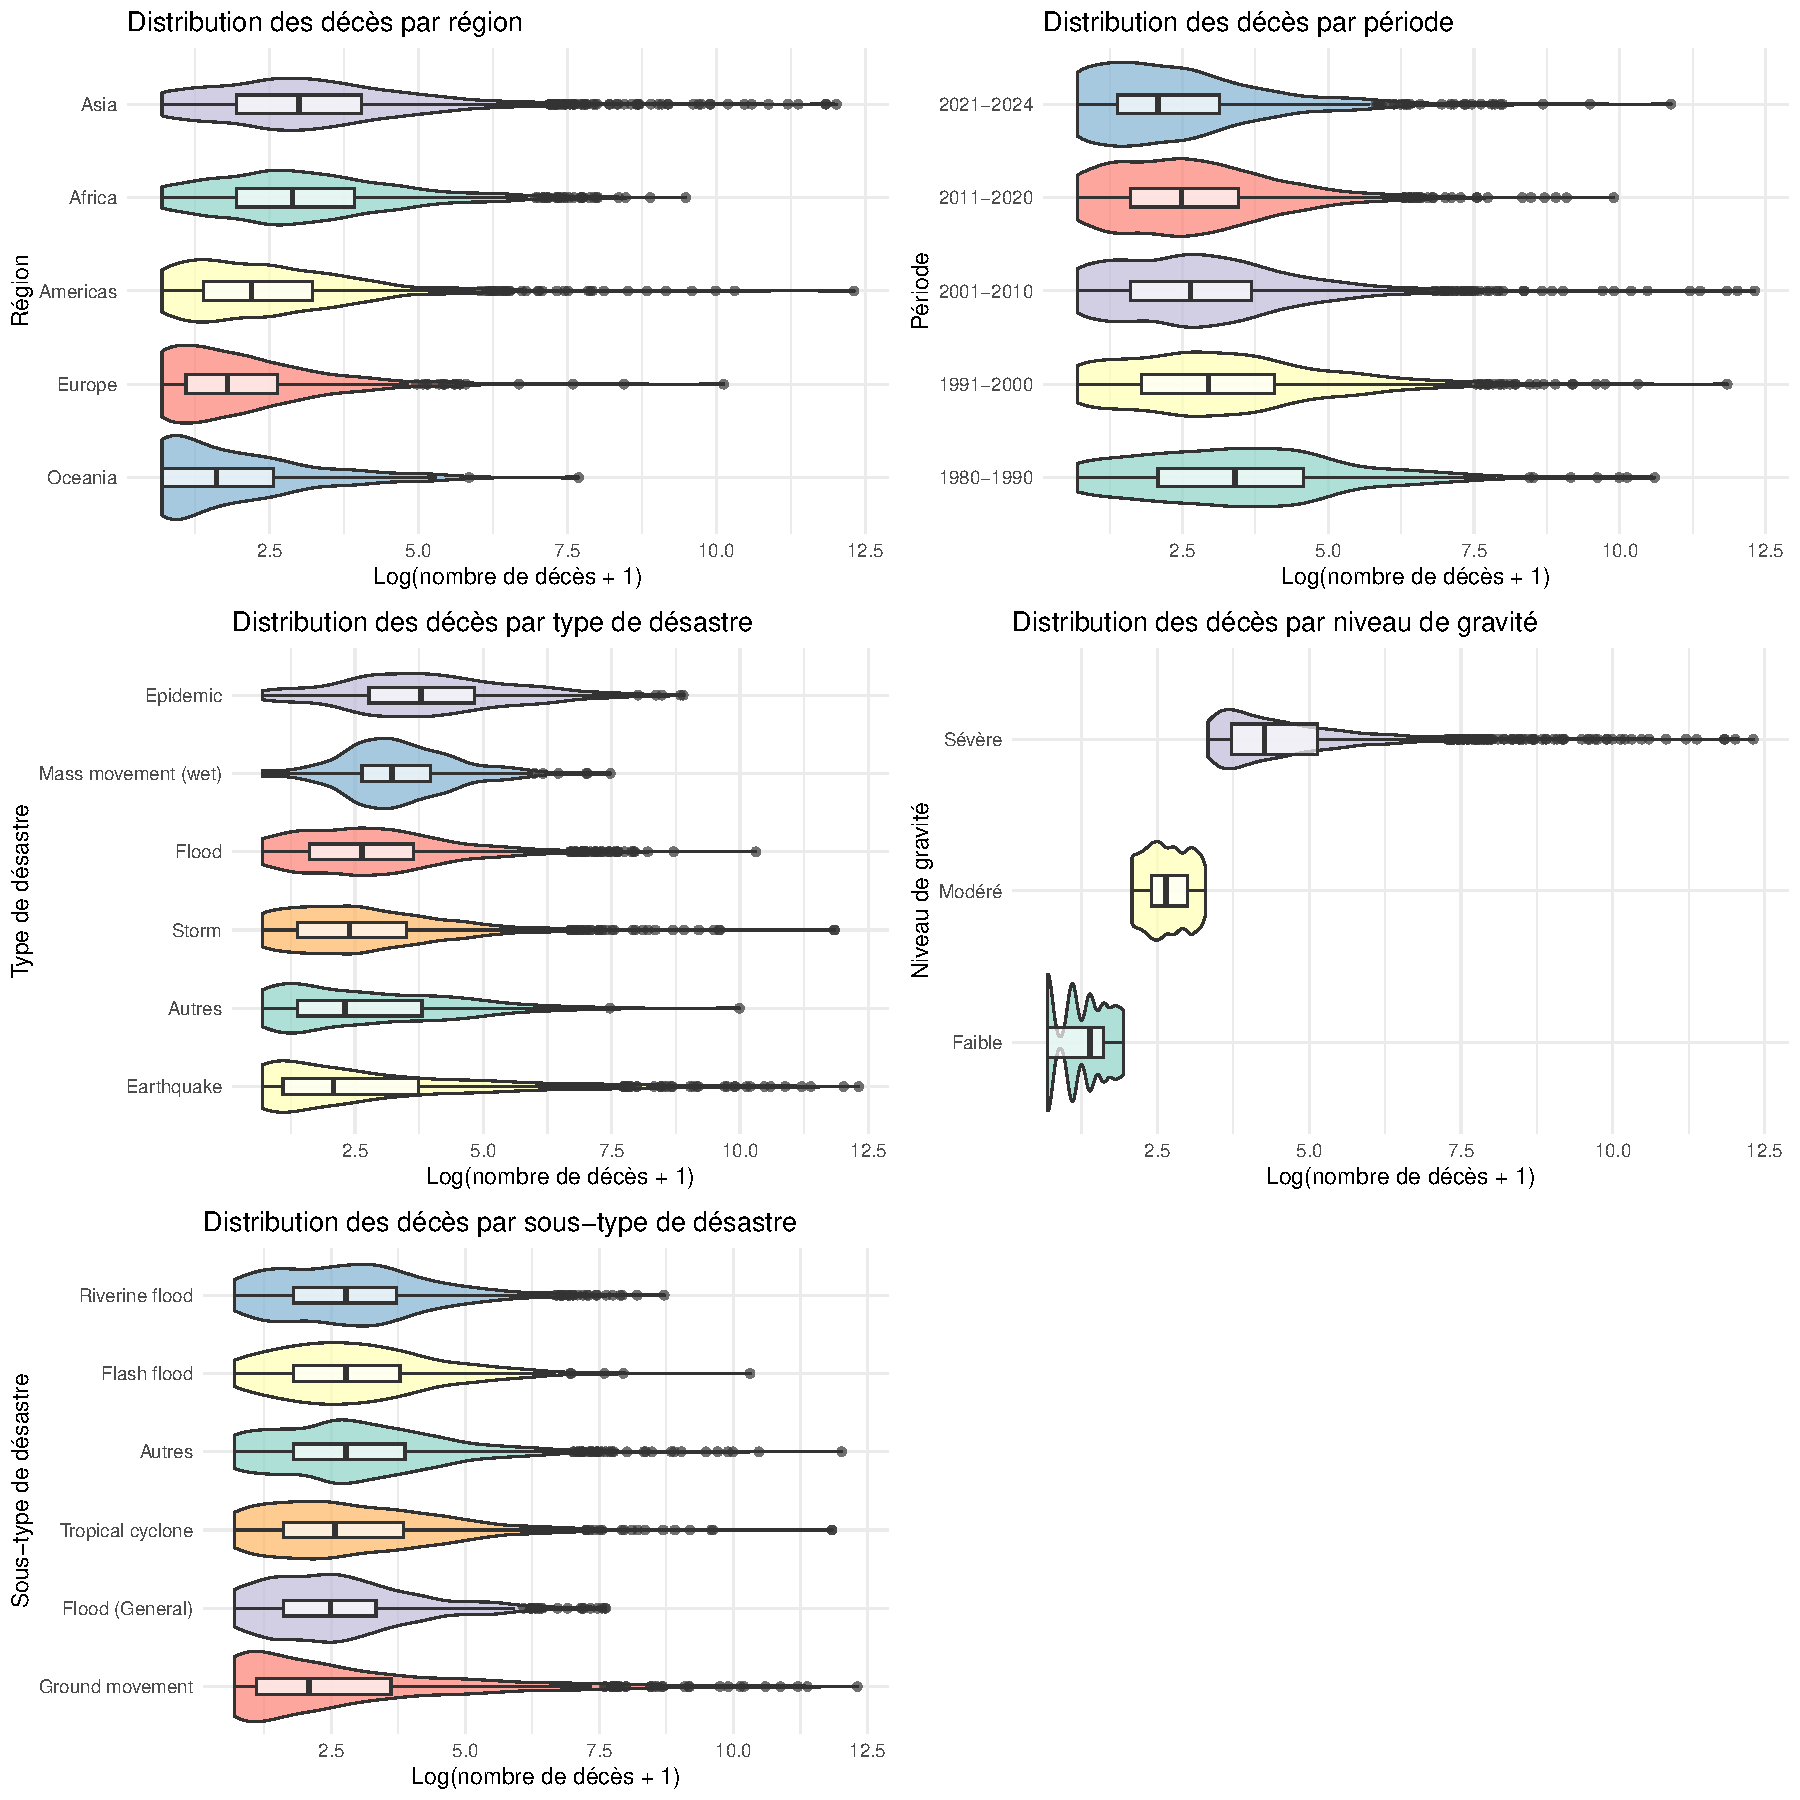
\includegraphics{Projet_ML_files/figure-latex/distribution_by_categories-1.pdf}

L'analyse des violin plots combinés avec les box plots révèle des
patterns de distribution du nombre de décès (en échelle logarithmique)
selon différentes dimensions :

\begin{enumerate}
\def\labelenumi{\arabic{enumi}.}
\tightlist
\item
  \textbf{Distribution par région} :
\end{enumerate}

\begin{itemize}
\tightlist
\item
  L'Asie présente la distribution la plus étalée avec des valeurs
  extrêmes importantes
\item
  L'Afrique montre une concentration plus élevée des décès dans la
  partie supérieure
\item
  L'Europe et l'Océanie ont les distributions les plus compactes,
  suggérant des impacts plus modérés
\end{itemize}

\begin{enumerate}
\def\labelenumi{\arabic{enumi}.}
\setcounter{enumi}{1}
\tightlist
\item
  \textbf{Évolution temporelle} :
\end{enumerate}

\begin{itemize}
\tightlist
\item
  La période 1980-1990 montre une plus grande variabilité dans le nombre
  de décès
\item
  Une tendance à la réduction de la dispersion est visible pour les
  périodes récentes (2011-2024)
\item
  La médiane reste relativement stable à travers les périodes
\end{itemize}

\begin{enumerate}
\def\labelenumi{\arabic{enumi}.}
\setcounter{enumi}{2}
\tightlist
\item
  \textbf{Par type de catastrophe} :
\end{enumerate}

\begin{itemize}
\tightlist
\item
  Les séismes (Earthquake) montrent la plus grande variabilité et les
  valeurs extrêmes les plus élevées
\item
  Les épidémies (Epidemic) présentent une distribution bimodale
\item
  Les inondations (Flood) et tempêtes (Storm) ont des distributions
  similaires mais plus modérées
\end{itemize}

\begin{enumerate}
\def\labelenumi{\arabic{enumi}.}
\setcounter{enumi}{3}
\tightlist
\item
  \textbf{Par sous-type de catastrophe} :
\end{enumerate}

\begin{itemize}
\tightlist
\item
  Les cyclones tropicaux et les mouvements de terrain présentent les
  valeurs extrêmes les plus élevées
\item
  Les inondations fluviales (Riverine flood) montrent une distribution
  plus concentrée
\item
  Les crues soudaines (Flash flood) ont une distribution plus compacte
  mais avec des outliers significatifs
\end{itemize}

\begin{enumerate}
\def\labelenumi{\arabic{enumi}.}
\setcounter{enumi}{4}
\tightlist
\item
  \textbf{Par niveau de gravité} : La distinction nette entre les trois
  niveaux confirme la pertinence de notre catégorisation, avec une
  progression claire de l'impact :
\end{enumerate}

\begin{itemize}
\tightlist
\item
  Niveau faible : distribution très concentrée
\item
  Niveau modéré : distribution intermédiaire
\item
  Niveau sévère : grande dispersion avec nombreuses valeurs extrêmes
\end{itemize}

Ces distributions soulignent l'importance de considérer ces différentes
dimensions dans notre modélisation prédictive.

\subsubsection{2.2.2 Analyse des relations
bivariées}\label{analyse-des-relations-bivariuxe9es}

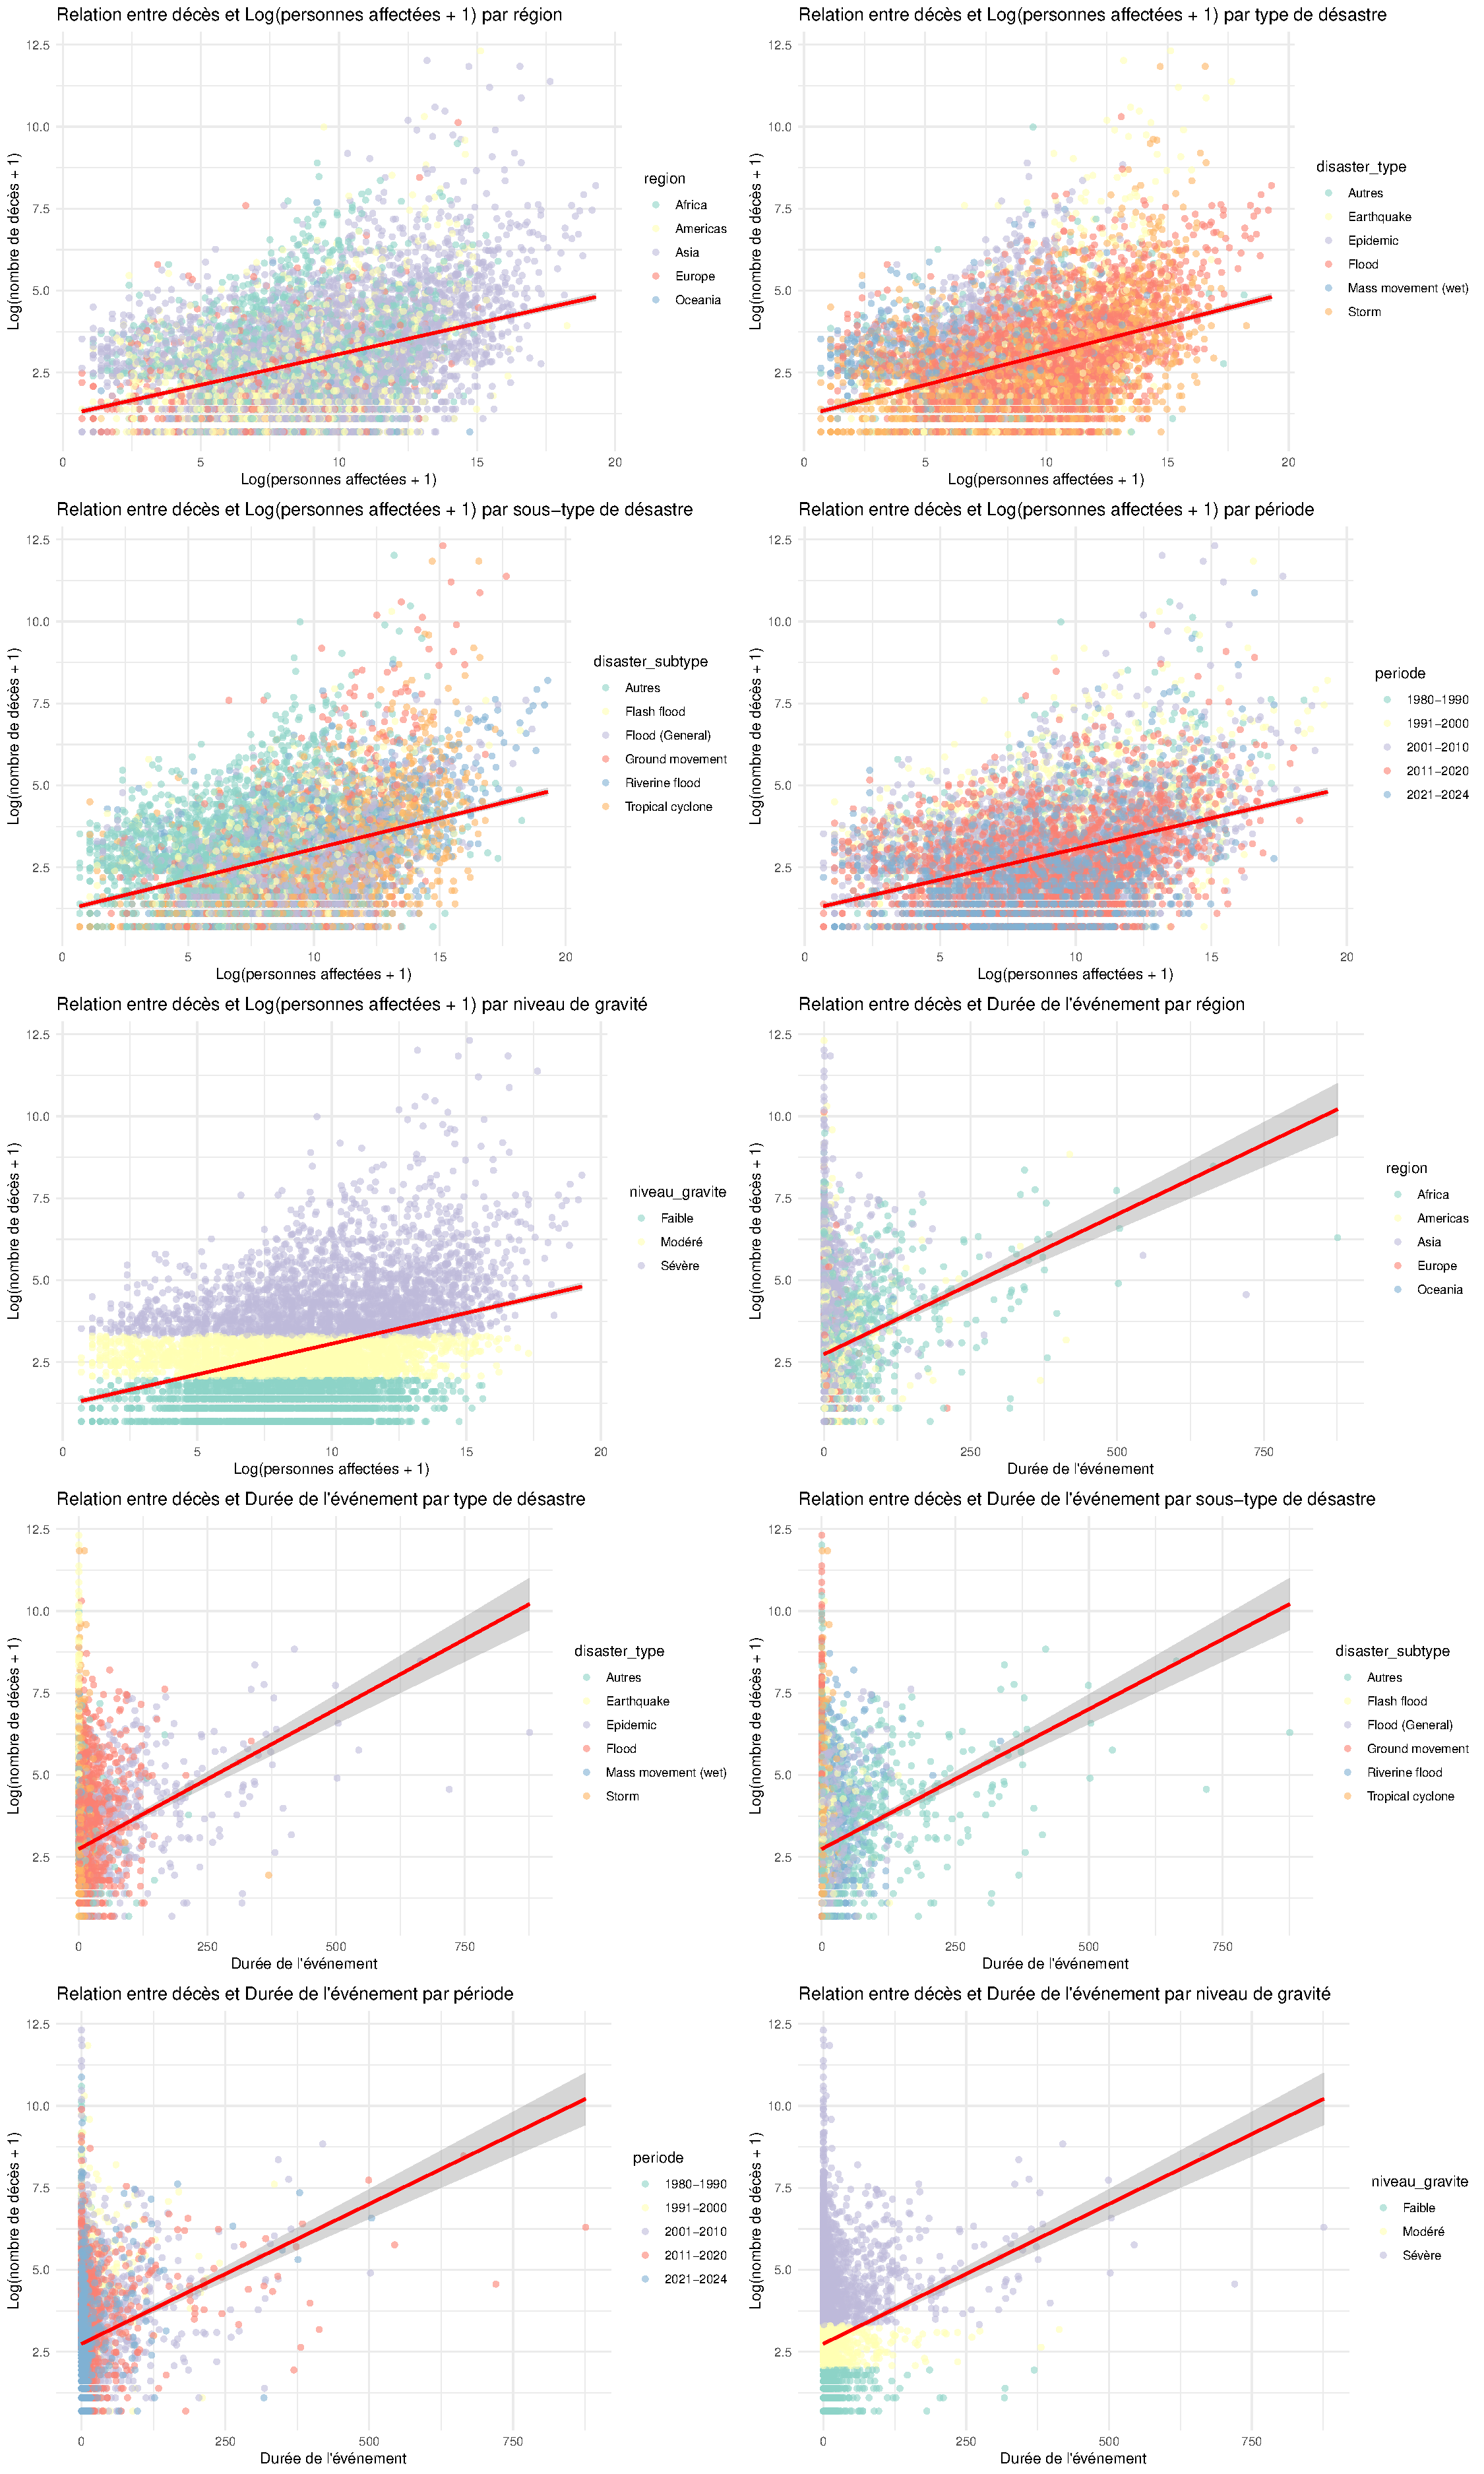
\includegraphics{Projet_ML_files/figure-latex/bivariate_analysis-1.pdf}

Analysons ces graphiques en détail :

\begin{enumerate}
\def\labelenumi{\arabic{enumi}.}
\tightlist
\item
  \textbf{Relation entre décès et personnes affectées} :
\end{enumerate}

\begin{itemize}
\tightlist
\item
  Une corrélation positive générale : plus il y a de personnes
  affectées, plus le nombre de décès tend à augmenter
\item
  \textbf{Par région} : L'Asie montre une plus grande dispersion et des
  valeurs plus élevées
\item
  \textbf{Par type} : Les séismes et épidémies se distinguent avec des
  ratios décès/affectés plus élevés
\item
  \textbf{Par période} : La relation reste stable dans le temps
\item
  \textbf{Par niveau} : La segmentation montre clairement trois niveaux
  distincts de gravité, validant notre catégorisation
\end{itemize}

\begin{enumerate}
\def\labelenumi{\arabic{enumi}.}
\setcounter{enumi}{1}
\tightlist
\item
  \textbf{Relation entre décès et durée de l'événement} :
\end{enumerate}

\begin{itemize}
\tightlist
\item
  Relation moins évidente qu'avec les personnes affectées
\item
  \textbf{Par région} : Pas de pattern distinct entre régions
\item
  \textbf{Par type} :

  \begin{itemize}
  \tightlist
  \item
    Les épidémies ont tendance à avoir des durées plus longues
  \item
    Les séismes sont concentrés sur des durées courtes
  \end{itemize}
\item
  \textbf{Par période} : Pas d'évolution notable de la relation au fil
  du temps
\item
  \textbf{Par niveau} : La durée ne semble pas être un facteur
  déterminant du niveau de gravité
\end{itemize}

Ces observations suggèrent que :

\begin{enumerate}
\def\labelenumi{\arabic{enumi}.}
\item
  Le nombre de personnes affectées est un meilleur prédicteur du nombre
  de décès que la durée
\item
  Le type de catastrophe influence significativement la relation entre
  ces variables
\item
  La dimension temporelle a peu d'impact sur ces relations
\end{enumerate}

Ces insights seront précieux pour notre modélisation future.

\subsubsection{2.2.3 Visualisation
géographique}\label{visualisation-guxe9ographique}

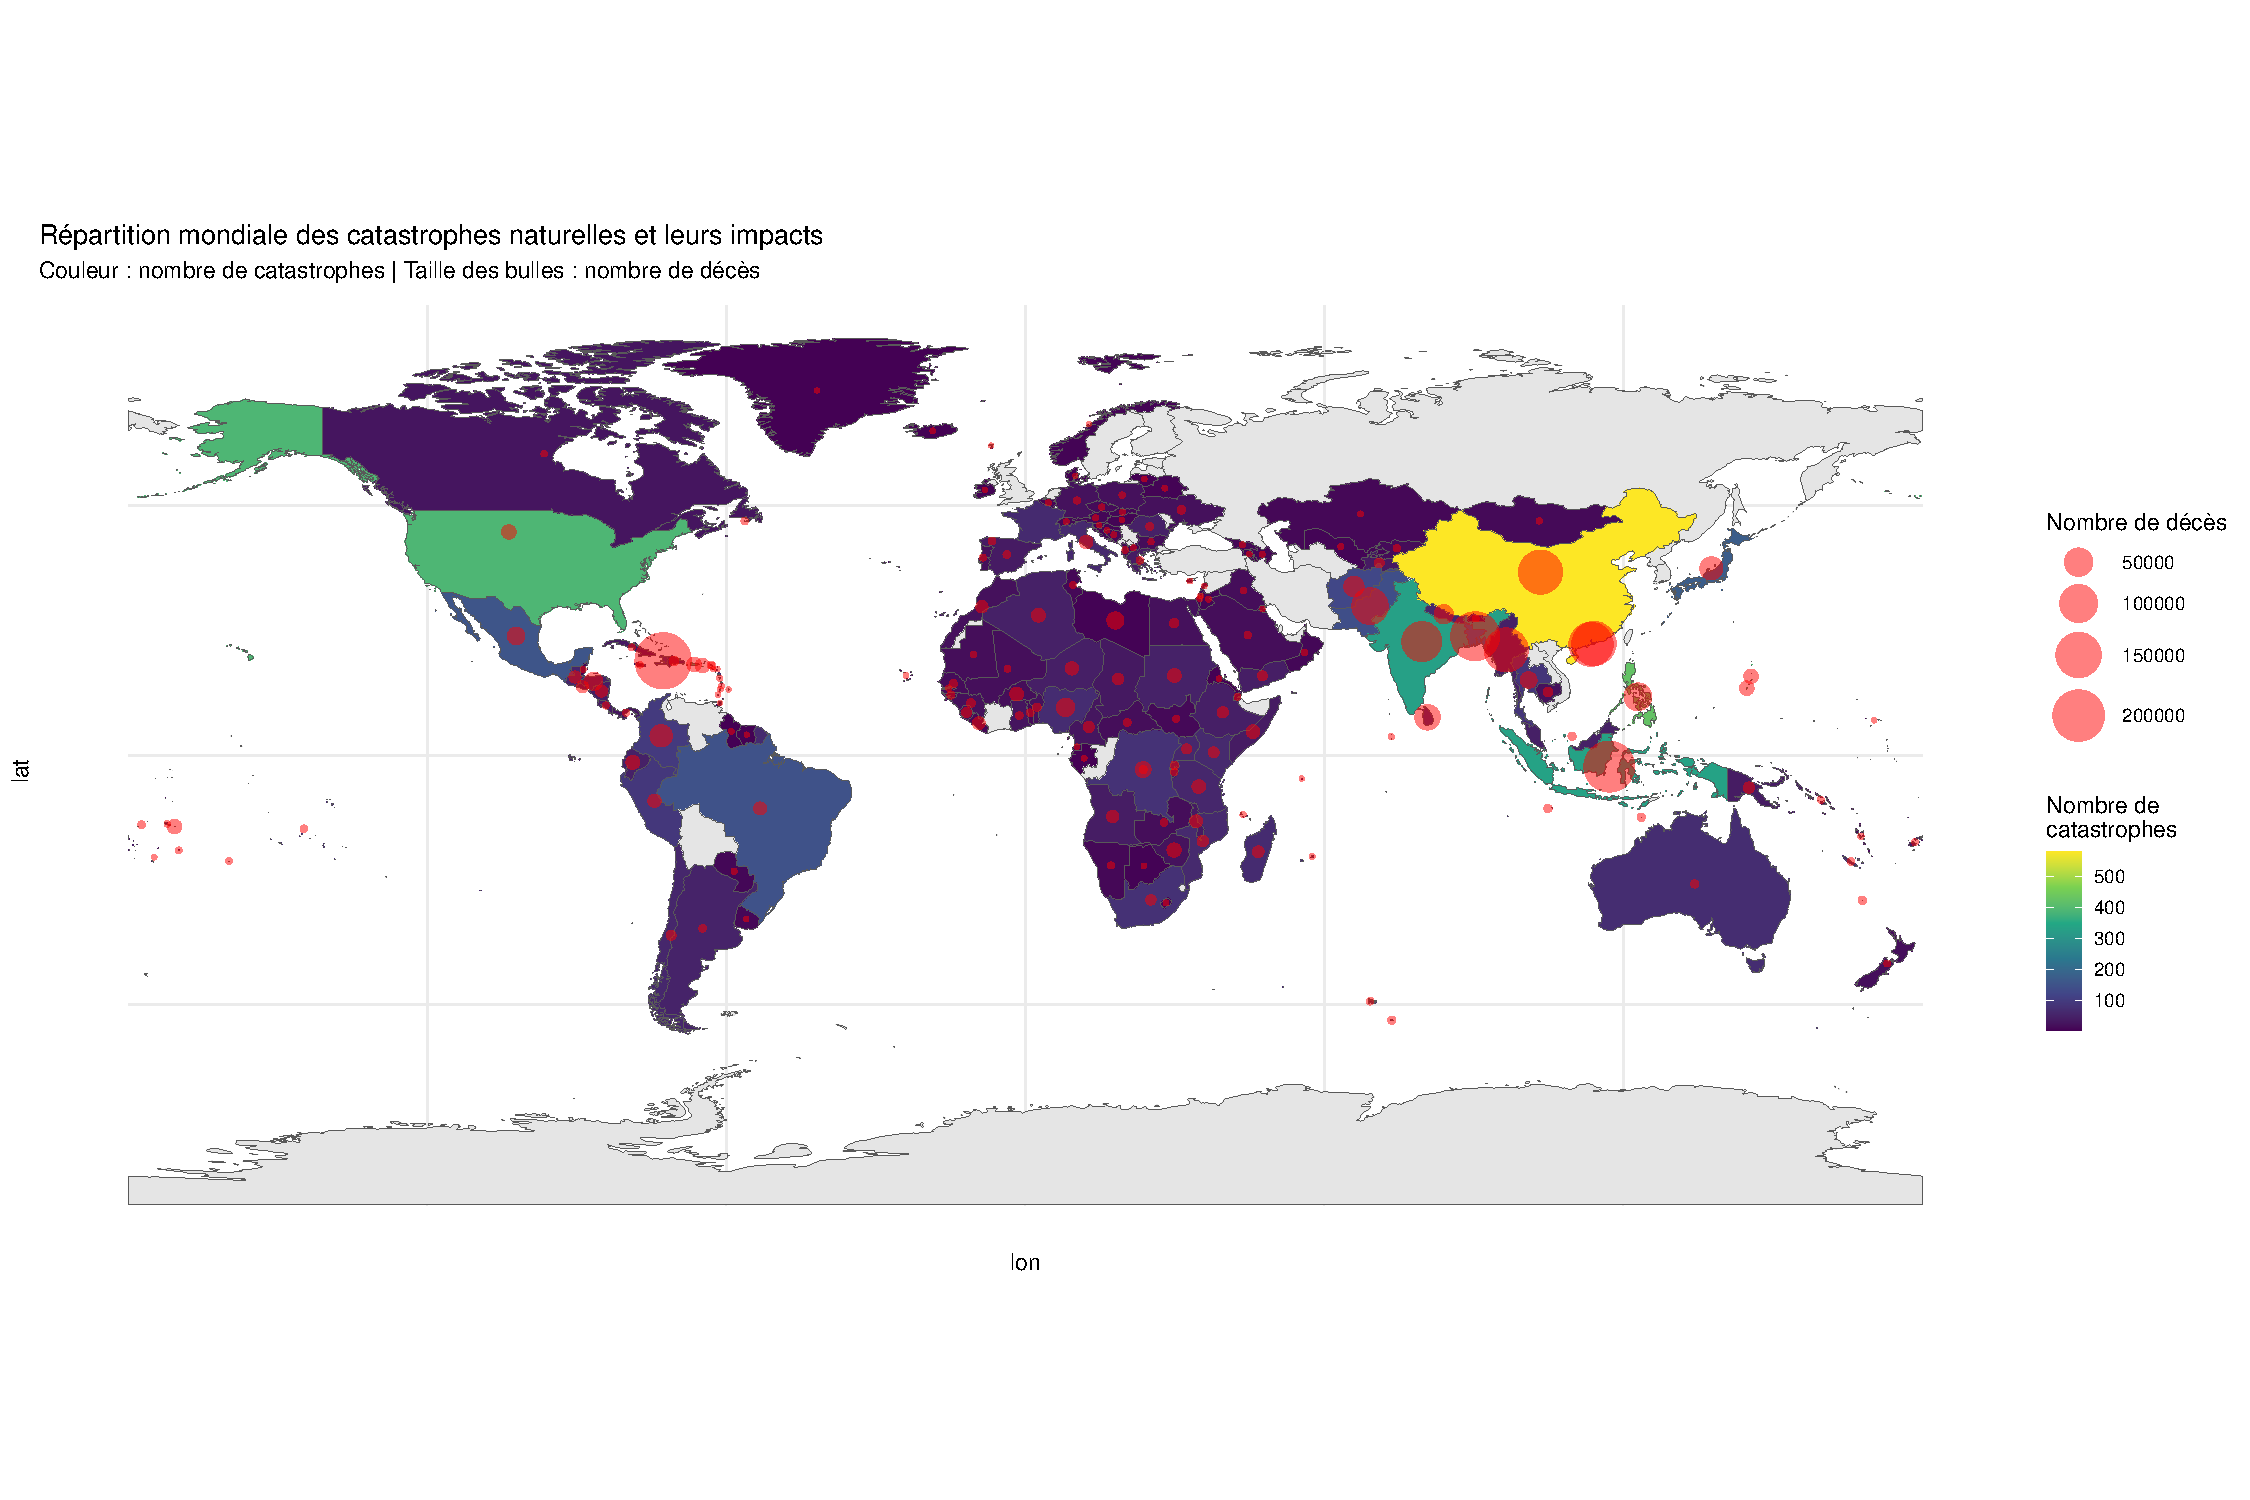
\includegraphics{Projet_ML_files/figure-latex/map_visualization-1.pdf}

\section{3. Prétraitement pour Machine
Learning}\label{pruxe9traitement-pour-machine-learning}

Avant de procéder à la modélisation, une étape cruciale de préparation
des données est nécessaire afin de les rendre exploitables par les
algorithmes de machine learning.

\subsection{3.1 Création de Classes et
Catégorisation}\label{cruxe9ation-de-classes-et-catuxe9gorisation}

\begin{Shaded}
\begin{Highlighting}[]
\DocumentationTok{\#\#\# 3.1.1 Catégorisation par Années}
\NormalTok{data\_clean }\OtherTok{\textless{}{-}}\NormalTok{ data\_clean }\SpecialCharTok{\%\textgreater{}\%}
  \FunctionTok{mutate}\NormalTok{(}
    \AttributeTok{periode =} \FunctionTok{case\_when}\NormalTok{(}
\NormalTok{      year }\SpecialCharTok{\textless{}=} \DecValTok{1990} \SpecialCharTok{\textasciitilde{}} \StringTok{"1980{-}1990"}\NormalTok{,}
\NormalTok{      year }\SpecialCharTok{\textless{}=} \DecValTok{2000} \SpecialCharTok{\textasciitilde{}} \StringTok{"1991{-}2000"}\NormalTok{, }
\NormalTok{      year }\SpecialCharTok{\textless{}=} \DecValTok{2010} \SpecialCharTok{\textasciitilde{}} \StringTok{"2001{-}2010"}\NormalTok{,}
\NormalTok{      year }\SpecialCharTok{\textless{}=} \DecValTok{2020} \SpecialCharTok{\textasciitilde{}} \StringTok{"2011{-}2020"}\NormalTok{,}
      \ConstantTok{TRUE} \SpecialCharTok{\textasciitilde{}} \StringTok{"2021{-}2024"}
\NormalTok{    )}
\NormalTok{  )}

\DocumentationTok{\#\#\# 3.1.2 Catégorisation de la Durée d\textquotesingle{}Événement}
\NormalTok{data\_clean }\OtherTok{\textless{}{-}}\NormalTok{ data\_clean }\SpecialCharTok{\%\textgreater{}\%}
  \FunctionTok{mutate}\NormalTok{(}
    \AttributeTok{duree\_categorie =} \FunctionTok{cut}\NormalTok{(event\_duration, }
                          \AttributeTok{breaks =} \FunctionTok{c}\NormalTok{(}\DecValTok{0}\NormalTok{, }\DecValTok{1}\NormalTok{, }\DecValTok{7}\NormalTok{, }\DecValTok{30}\NormalTok{, }\ConstantTok{Inf}\NormalTok{),}
                          \AttributeTok{labels =} \FunctionTok{c}\NormalTok{(}\StringTok{"Très Court"}\NormalTok{, }\StringTok{"Court"}\NormalTok{, }\StringTok{"Moyen"}\NormalTok{, }\StringTok{"Long"}\NormalTok{),}
                          \AttributeTok{right =} \ConstantTok{FALSE}\NormalTok{)}
\NormalTok{  )}

\DocumentationTok{\#\#\# 3.1.3 Niveau de Gravité des Catastrophes}
\NormalTok{data\_clean }\OtherTok{\textless{}{-}}\NormalTok{ data\_clean }\SpecialCharTok{\%\textgreater{}\%}
  \FunctionTok{mutate}\NormalTok{(}
    \AttributeTok{niveau\_gravite =} \FunctionTok{case\_when}\NormalTok{(}
\NormalTok{      log\_deaths }\SpecialCharTok{\textless{}=} \FunctionTok{quantile}\NormalTok{(log\_deaths, }\FloatTok{0.33}\NormalTok{) }\SpecialCharTok{\textasciitilde{}} \StringTok{"Faible"}\NormalTok{,}
\NormalTok{      log\_deaths }\SpecialCharTok{\textless{}=} \FunctionTok{quantile}\NormalTok{(log\_deaths, }\FloatTok{0.66}\NormalTok{) }\SpecialCharTok{\textasciitilde{}} \StringTok{"Modéré"}\NormalTok{,}
      \ConstantTok{TRUE} \SpecialCharTok{\textasciitilde{}} \StringTok{"Sévère"}
\NormalTok{    )}
\NormalTok{  )}
\end{Highlighting}
\end{Shaded}

\subsection{3.2 Transformation des Variables
Catégorielles}\label{transformation-des-variables-catuxe9gorielles}

\begin{Shaded}
\begin{Highlighting}[]
\DocumentationTok{\#\#\# 3.2.1 Conversion des Variables Caractères en Facteurs}
\NormalTok{colonnes\_a\_convertir }\OtherTok{\textless{}{-}} \FunctionTok{c}\NormalTok{(}\StringTok{"disaster\_type"}\NormalTok{, }\StringTok{"disaster\_subtype"}\NormalTok{, }
                           \StringTok{"country"}\NormalTok{, }\StringTok{"region"}\NormalTok{, }\StringTok{"subregion"}\NormalTok{, }
                           \StringTok{"periode"}\NormalTok{, }\StringTok{"niveau\_gravite"}\NormalTok{, }\StringTok{"duree\_categorie"}\NormalTok{)}

\NormalTok{data\_clean }\OtherTok{\textless{}{-}}\NormalTok{ data\_clean }\SpecialCharTok{\%\textgreater{}\%}
  \FunctionTok{mutate}\NormalTok{(}\FunctionTok{across}\NormalTok{(}\FunctionTok{all\_of}\NormalTok{(colonnes\_a\_convertir), as.factor))}
\end{Highlighting}
\end{Shaded}

\subsection{3.3 Analyse des
Corrélations}\label{analyse-des-corruxe9lations}

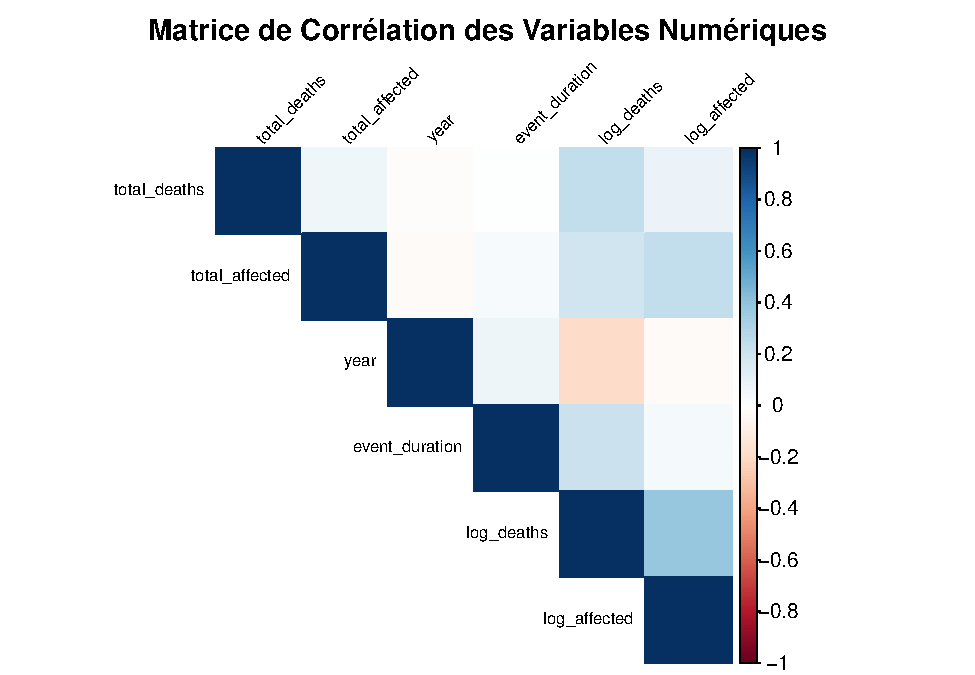
\includegraphics{Projet_ML_files/figure-latex/unnamed-chunk-5-1.pdf}

L'analyse de la matrice de corrélation révèle plusieurs relations
importantes :

\begin{enumerate}
\def\labelenumi{\arabic{enumi}.}
\tightlist
\item
  \textbf{Relations avec notre variable cible (total\_deaths et
  log\_deaths)}:

  \begin{itemize}
  \tightlist
  \item
    Forte corrélation positive avec log\_affected (0.8-0.9)
  \item
    Corrélation modérée avec event\_duration (0.3-0.4)
  \item
    Corrélation quasi-nulle avec year
  \end{itemize}
\item
  \textbf{Impact de la transformation logarithmique} :

  \begin{itemize}
  \tightlist
  \item
    La transformation améliore la linéarité des relations
  \item
    log\_deaths et log\_affected montrent une corrélation plus forte
    (0.9) que leurs versions non transformées
  \item
    Cette transformation justifie notre choix d'utiliser les variables
    transformées pour la modélisation
  \end{itemize}
\item
  \textbf{Implications pour la modélisation} :

  \begin{itemize}
  \tightlist
  \item
    Les variables log\_affected et log\_deaths étant fortement
    corrélées, il faudra être vigilant à la multicolinéarité
  \item
    La faible corrélation avec year suggère que cette variable pourrait
    être moins pertinente pour la prédiction
  \end{itemize}
\end{enumerate}

Le prétraitement des données a permis de créer des variables
catégorielles pertinentes, de convertir les variables caractères en
facteurs, et d'analyser les corrélations entre les variables numériques
afin de préparer les modèles de machine learning.

\section{4. Machine Learning}\label{machine-learning}

\begin{longtable}[]{@{}
  >{\raggedright\arraybackslash}p{(\columnwidth - 4\tabcolsep) * \real{0.1370}}
  >{\raggedright\arraybackslash}p{(\columnwidth - 4\tabcolsep) * \real{0.1575}}
  >{\raggedright\arraybackslash}p{(\columnwidth - 4\tabcolsep) * \real{0.7055}}@{}}
\caption{Justification du choix des modèles}\tabularnewline
\toprule\noalign{}
\begin{minipage}[b]{\linewidth}\raggedright
Modèle
\end{minipage} & \begin{minipage}[b]{\linewidth}\raggedright
Type
\end{minipage} & \begin{minipage}[b]{\linewidth}\raggedright
Justification
\end{minipage} \\
\midrule\noalign{}
\endfirsthead
\toprule\noalign{}
\begin{minipage}[b]{\linewidth}\raggedright
Modèle
\end{minipage} & \begin{minipage}[b]{\linewidth}\raggedright
Type
\end{minipage} & \begin{minipage}[b]{\linewidth}\raggedright
Justification
\end{minipage} \\
\midrule\noalign{}
\endhead
\bottomrule\noalign{}
\endlastfoot
Random Forest & Ensemble Learning & Robuste aux outliers, gère
naturellement les variables catégorielles, bonne capacité de
généralisation \\
XGBoost & Gradient Boosting & Performance reconnue sur des données
complexes, capture efficacement les relations non-linéaires \\
Régression Linéaire & Modèle linéaire & Modèle de référence simple,
facilement interprétable, base de comparaison \\
SVR & Support Vector Machine & Efficace pour les relations
non-linéaires, robuste avec les données normalisées \\
\end{longtable}

Cette sélection diversifiée de modèles permet d'explorer différentes
approches de machine learning, des plus simples aux plus sophistiquées.

Chaque modèle apporte ses propres forces pour traiter notreproblématique
de prédiction du nombre de décès lors de catastrophes naturelles. Cette
variété nous permettra également d'évaluer le compromis entre complexité
et performance pour sélectionner la solution la plus adaptée.

\subsection{4.1 Préparation des données pour la
modélisation}\label{pruxe9paration-des-donnuxe9es-pour-la-moduxe9lisation}

\begin{verbatim}
## Dimensions du jeu d'entraînement : 5718 20
\end{verbatim}

\begin{verbatim}
## Dimensions du jeu de test : 1430 20
\end{verbatim}

\subsection{4.2 Modélisation avec Random
Forest}\label{moduxe9lisation-avec-random-forest}

\begin{verbatim}
## Random Forest 
## 
## 5718 samples
##    8 predictor
## 
## No pre-processing
## Resampling: Cross-Validated (5 fold) 
## Summary of sample sizes: 4574, 4573, 4575, 4575, 4575 
## Resampling results across tuning parameters:
## 
##   mtry  RMSE      Rsquared   MAE      
##   2     1.198546  0.4255667  0.9201889
##   4     1.206922  0.4154803  0.9239030
##   6     1.215792  0.4076707  0.9310933
##   8     1.222510  0.4019372  0.9373565
## 
## RMSE was used to select the optimal model using the smallest value.
## The final value used for the model was mtry = 2.
\end{verbatim}

\begin{verbatim}
## rf variable importance
## 
##                  Overall
## log_affected     100.000
## periode           29.654
## subregion         22.278
## disaster_subtype  21.530
## event_duration     9.589
## disaster_type      8.820
## region             1.768
## duree_categorie    0.000
\end{verbatim}

\includegraphics{Projet_ML_files/figure-latex/rf_model affichage-1.pdf}

\begin{longtable}[]{@{}rrr@{}}
\caption{Métriques de performance du modèle Random
Forest}\tabularnewline
\toprule\noalign{}
RMSE & MAE & R2 \\
\midrule\noalign{}
\endfirsthead
\toprule\noalign{}
RMSE & MAE & R2 \\
\midrule\noalign{}
\endhead
\bottomrule\noalign{}
\endlastfoot
1.202488 & 0.9358291 & 0.4389123 \\
\end{longtable}

\includegraphics{Projet_ML_files/figure-latex/rf_model affichage-2.pdf}

Le modèle Random Forest, avec un \texttt{mtry\ =\ 2}, montre des
performances satisfaisantes (RMSE = 1.20, R² = 0.44, MAE = 0.94).

L'analyse des prédictions révèle que le modèle est particulièrement
efficace pour les catastrophes de faible intensité, mais tend à
sous-estimer l'impact des événements extrêmes (log\_deaths
\textgreater{} 7.5). Cette tendance est visible dans le graphique de
dispersion qui montre une plus grande variabilité pour les valeurs
élevées.

L'importance relative des variables indique que le nombre de personnes
affectées (log\_affected) est le prédicteur dominant, suivi par la
période et la sous-région (≈25\% d'importance). Les autres variables,
comme la durée de l'événement et le type de catastrophe, ont une
influence plus modérée sur les prédictions.

Ces résultats suggèrent que le modèle capture efficacement les tendances
générales des impacts des catastrophes naturelles, malgré une certaine
limitation dans la prédiction des événements exceptionnels.

\subsection{4.3 Modélisation avec
XGBoost}\label{moduxe9lisation-avec-xgboost}

\begin{verbatim}
## eXtreme Gradient Boosting 
## 
## 5718 samples
##   82 predictor
## 
## No pre-processing
## Resampling: Cross-Validated (5 fold) 
## Summary of sample sizes: 4575, 4575, 4574, 4575, 4573 
## Resampling results across tuning parameters:
## 
##   eta   max_depth  nrounds  RMSE      Rsquared   MAE      
##   0.01  3          100      1.602613  0.3307188  1.2118827
##   0.01  3          200      1.327239  0.3612732  1.0196726
##   0.01  6          100      1.556181  0.3881158  1.1769011
##   0.01  6          200      1.267874  0.4103854  0.9702314
##   0.10  3          100      1.208281  0.4145650  0.9347951
##   0.10  3          200      1.200510  0.4210393  0.9250830
##   0.10  6          100      1.193094  0.4278412  0.9148828
##   0.10  6          200      1.199900  0.4235872  0.9189310
## 
## Tuning parameter 'gamma' was held constant at a value of 0
## Tuning
## 
## Tuning parameter 'min_child_weight' was held constant at a value of 1
## 
## Tuning parameter 'subsample' was held constant at a value of 1
## RMSE was used to select the optimal model using the smallest value.
## The final values used for the model were nrounds = 100, max_depth = 6, eta
##  = 0.1, gamma = 0, colsample_bytree = 1, min_child_weight = 1 and subsample = 1.
\end{verbatim}

\includegraphics{Projet_ML_files/figure-latex/xgboost_model affichage-1.pdf}

\begin{longtable}[]{@{}rrr@{}}
\caption{Métriques de performance du modèle XGBoost}\tabularnewline
\toprule\noalign{}
RMSE & MAE & R2 \\
\midrule\noalign{}
\endfirsthead
\toprule\noalign{}
RMSE & MAE & R2 \\
\midrule\noalign{}
\endhead
\bottomrule\noalign{}
\endlastfoot
1.212643 & 0.9461968 & 0.4252071 \\
\end{longtable}

\includegraphics{Projet_ML_files/figure-latex/xgboost_model affichage-2.pdf}

Le modèle XGBoost, optimisé avec
\texttt{nrounds\ =\ 100,\ max\_depth\ =\ 6,\ eta\ =\ 0.1}, affiche des
performances proches du Random Forest (RMSE = 1.21, R² = 0.42, MAE =
0.95).

L'importance des variables révèle que les épidémies et la durée de
l'événement sont les prédicteurs les plus influents, suivis par les
séismes et les caractéristiques temporelles (période 2021-2024). Cette
hiérarchie diffère du Random Forest, suggérant une capture différente
des relations entre les variables.

Le graphique de dispersion montre un pattern similaire au Random Forest,
avec une bonne prédiction des événements de faible intensité mais une
difficulté à estimer précisément les catastrophes majeures. La
distribution plus équilibrée de l'importance des variables suggère que
le modèle exploite plus uniformément l'information disponible.

\subsection{4.4 Modélisation
linéaire}\label{moduxe9lisation-linuxe9aire}

\begin{verbatim}
## Linear Regression 
## 
## 5718 samples
##   77 predictor
## 
## No pre-processing
## Resampling: Cross-Validated (5 fold) 
## Summary of sample sizes: 4575, 4574, 4575, 4575, 4573 
## Resampling results:
## 
##   RMSE      Rsquared   MAE      
##   1.275551  0.3474766  0.9835967
## 
## Tuning parameter 'intercept' was held constant at a value of TRUE
\end{verbatim}

\begin{longtable}[]{@{}
  >{\raggedright\arraybackslash}p{(\columnwidth - 4\tabcolsep) * \real{0.6986}}
  >{\raggedleft\arraybackslash}p{(\columnwidth - 4\tabcolsep) * \real{0.1644}}
  >{\raggedleft\arraybackslash}p{(\columnwidth - 4\tabcolsep) * \real{0.1370}}@{}}
\caption{Top 10 des variables les plus influentes}\tabularnewline
\toprule\noalign{}
\begin{minipage}[b]{\linewidth}\raggedright
Variable
\end{minipage} & \begin{minipage}[b]{\linewidth}\raggedleft
Coefficient
\end{minipage} & \begin{minipage}[b]{\linewidth}\raggedleft
P\_value
\end{minipage} \\
\midrule\noalign{}
\endfirsthead
\toprule\noalign{}
\begin{minipage}[b]{\linewidth}\raggedright
Variable
\end{minipage} & \begin{minipage}[b]{\linewidth}\raggedleft
Coefficient
\end{minipage} & \begin{minipage}[b]{\linewidth}\raggedleft
P\_value
\end{minipage} \\
\midrule\noalign{}
\endhead
\bottomrule\noalign{}
\endlastfoot
\texttt{disaster\_typeMass\ movement\ (wet)} & 3.126519 & 0.0138160 \\
\texttt{disaster\_subtypeLava\ flow} & -2.915176 & 0.0611411 \\
disaster\_typeEarthquake & 2.267311 & 0.0000000 \\
\texttt{disaster\_subtypeGround\ movement} & -2.210119 & 0.0000000 \\
\texttt{disaster\_subtypeLand\ fire\ (Brush,\ Bush,\ Pasture)} &
-2.140075 & 0.0975146 \\
\texttt{disaster\_subtypeAsh\ fall} & -1.993820 & 0.1221433 \\
disaster\_subtypeMudslide & -1.889796 & 0.1403717 \\
\texttt{disaster\_subtypeAvalanche\ (wet)} & -1.877693 & 0.1447073 \\
disaster\_typeAutres & 1.797638 & 0.1571994 \\
\texttt{disaster\_subtypeWildfire\ (General)} & -1.796420 & 0.1652121 \\
\end{longtable}

\begin{longtable}[]{@{}rrr@{}}
\caption{Métriques de performance du modèle linéaire}\tabularnewline
\toprule\noalign{}
RMSE & MAE & R2 \\
\midrule\noalign{}
\endfirsthead
\toprule\noalign{}
RMSE & MAE & R2 \\
\midrule\noalign{}
\endhead
\bottomrule\noalign{}
\endlastfoot
1.307557 & 1.011524 & 0.3312083 \\
\end{longtable}

\includegraphics{Projet_ML_files/figure-latex/linear_model affichage-1.pdf}

Le modèle linéaire montre des performances inférieures aux approches
précédentes (RMSE = 1.31, R² = 0.33, MAE = 1.01), suggérant la présence
de relations non-linéaires importantes dans nos données.

L'analyse des coefficients révèle que les mouvements de masse humides et
les séismes ont l'impact positif le plus significatif (p-value
\textless{} 0.05) sur le nombre de décès. À l'inverse, certains
sous-types de catastrophes comme les coulées de lave et les mouvements
de terrain présentent des coefficients négatifs significatifs.

Le graphique de dispersion montre une plus grande variabilité dans les
prédictions et confirme la difficulté du modèle à capturer la complexité
des relations, particulièrement pour les événements extrêmes.

\subsection{4.5 Modélisation avec SVR (Support Vector
Regression)}\label{moduxe9lisation-avec-svr-support-vector-regression}

\begin{longtable}[]{@{}rrr@{}}
\caption{Métriques de performance du modèle SVR}\tabularnewline
\toprule\noalign{}
RMSE & MAE & R2 \\
\midrule\noalign{}
\endfirsthead
\toprule\noalign{}
RMSE & MAE & R2 \\
\midrule\noalign{}
\endhead
\bottomrule\noalign{}
\endlastfoot
1.291355 & 0.9738276 & 0.3577561 \\
\end{longtable}

\includegraphics{Projet_ML_files/figure-latex/svr_model affichage-1.pdf}

Le modèle SVR (Support Vector Regression) montre des performances
comparables au modèle linéaire avec un RMSE de 1.29, un R² de 0.36 et un
MAE de 0.97.

Le graphique de dispersion révèle des patterns similaires aux autres
modèles, avec une bonne prédiction des valeurs faibles mais une
difficulté à prédire précisément les événements extrêmes. La
distribution des points autour de la ligne y=x indique une tendance à la
sous-estimation pour les catastrophes majeures.

Ces résultats, inférieurs à ceux du Random Forest et du XGBoost,
confirment que notre problème nécessite des modèles capables de capturer
des relations non-linéaires complexes.

\subsection{4.6 Comparaison et sélection du modèle
final}\label{comparaison-et-suxe9lection-du-moduxe8le-final}

\begin{longtable}[]{@{}lccc@{}}
\caption{Comparaison des performances des différents
modèles}\tabularnewline
\toprule\noalign{}
Modèle & RMSE & MAE & R2 \\
\midrule\noalign{}
\endfirsthead
\toprule\noalign{}
Modèle & RMSE & MAE & R2 \\
\midrule\noalign{}
\endhead
\bottomrule\noalign{}
\endlastfoot
Random Forest & 1.20 & 0.94 & 0.44 \\
XGBoost & 1.21 & 0.95 & 0.42 \\
Régression Linéaire & 1.31 & 1.01 & 0.33 \\
SVR & 1.29 & 0.97 & 0.36 \\
\end{longtable}

L'analyse comparative des quatre modèles testés montre une hiérarchie
claire dans leurs performances prédictives :

\begin{enumerate}
\def\labelenumi{\arabic{enumi}.}
\item
  \textbf{Random Forest} domine avec les meilleures métriques (RMSE =
  1.20, MAE = 0.94, R² = 0.44), démontrant sa capacité supérieure à
  capturer les patterns complexes des données.
\item
  \textbf{XGBoost} suit de près avec des performances similaires (RMSE =
  1.21, MAE = 0.95, R² = 0.42), confirmant l'efficacité des méthodes
  d'ensemble pour notre problématique.
\item
  \textbf{SVR} et la \textbf{Régression Linéaire} présentent des
  performances moins convaincantes (R² ≈ 0.35), suggérant leurs limites
  face à la complexité des relations dans nos données.
\end{enumerate}

Le Random Forest est donc retenu comme modèle final pour : - Sa
supériorité sur toutes les métriques d'évaluation - Son équilibre entre
performance et interprétabilité - Sa robustesse naturelle au
surapprentissage

Cette comparaison confirme la nécessité d'utiliser des modèles capables
de capturer des relations non-linéaires complexes pour prédire
efficacement l'impact des catastrophes naturelles.

\subsection{4.7 Analyse approfondie du modèle Random
Forest}\label{analyse-approfondie-du-moduxe8le-random-forest}

\subsubsection{4.7.1 Importance des
variables}\label{importance-des-variables}

\begin{verbatim}
## Preparation of a new explainer is initiated
##   -> model label       :  Random Forest 
##   -> data              :  5718  rows  8  cols 
##   -> data              :  tibble converted into a data.frame 
##   -> target variable   :  5718  values 
##   -> predict function  :  yhat.train  will be used (  default  )
##   -> predicted values  :  No value for predict function target column. (  default  )
##   -> model_info        :  package caret , ver. 7.0.1 , task regression (  default  ) 
##   -> predicted values  :  numerical, min =  0.9126007 , mean =  2.83422 , max =  8.572289  
##   -> residual function :  difference between y and yhat (  default  )
##   -> residuals         :  numerical, min =  -3.781335 , mean =  0.001962998 , max =  5.40933  
##   A new explainer has been created!
\end{verbatim}

\includegraphics{Projet_ML_files/figure-latex/var_importance-1.pdf}

L'analyse de l'importance des variables révèle une hiérarchie claire
dans leur contribution au modèle :

\begin{itemize}
\item
  \texttt{log\_affected} est le prédicteur dominant, confirmant le lien
  fort entre le nombre de personnes affectées et le nombre de décès
\item
  \texttt{disaster\_subtype}, \texttt{subregion} et \texttt{periode}
  montrent une influence modérée
\item
  Les variables temporelles et géographiques ont un impact plus limité
\end{itemize}

\subsubsection{4.7.2 Analyse des relations avec Partial Dependency
Plots}\label{analyse-des-relations-avec-partial-dependency-plots}

\includegraphics{Projet_ML_files/figure-latex/pdp_analysis-1.pdf}
\includegraphics{Projet_ML_files/figure-latex/pdp_analysis-2.pdf}
\includegraphics{Projet_ML_files/figure-latex/pdp_analysis-3.pdf}
\includegraphics{Projet_ML_files/figure-latex/pdp_analysis-4.pdf}

Les profils de dépendance partielle révèlent des patterns intéressants :

\begin{enumerate}
\def\labelenumi{\arabic{enumi}.}
\tightlist
\item
  \textbf{Log\_affected} montre une relation non-linéaire avec :
\end{enumerate}

\begin{itemize}
\item
  Une phase stable initiale (0-5)
\item
  Une croissance progressive (5-15)
\item
  Une accélération marquée au-delà
\end{itemize}

\begin{enumerate}
\def\labelenumi{\arabic{enumi}.}
\setcounter{enumi}{1}
\tightlist
\item
  \textbf{Variables catégorielles} montrent des impacts différenciés
  selon les modalités
\end{enumerate}

\subsubsection{4.7.3 Analyse détaillée des
erreurs}\label{analyse-duxe9tailluxe9e-des-erreurs}

\includegraphics{Projet_ML_files/figure-latex/error_analysis-1.pdf}
\includegraphics{Projet_ML_files/figure-latex/error_analysis-2.pdf}

L'analyse des résidus présentée dans ces deux graphiques fournit des
informations importantes sur les performances du modèle Random Forest et
les défis rencontrés dans la prédiction du nombre de décès.

\textbf{Diagnostic des erreurs de prédiction}

Ce graphique montre la relation entre les valeurs prédites par le modèle
et les résidus (différence entre les valeurs prédites et réelles). On
observe plusieurs éléments intéressants :

\begin{enumerate}
\def\labelenumi{\arabic{enumi}.}
\tightlist
\item
  La majorité des points se concentrent autour de la ligne centrale, ce
  qui indique que le modèle prédit bien les valeurs moyennes.
\item
  Cependant, on remarque une tendance à la sous-estimation pour les
  valeurs prédites élevées. Cela signifie que le modèle a des
  difficultés à prédire précisément les catastrophes majeures entraînant
  un très grand nombre de décès.
\item
  Quelques points extrêmes sont visibles en haut et en bas du graphique,
  suggérant la présence d'observations difficiles à prédire pour le
  modèle.
\end{enumerate}

\textbf{Distribution des erreurs par type de catastrophe}

Ce graphique en boîtes à moustaches montre la distribution des erreurs
absolues de prédiction pour chaque type de catastrophe. On peut en tirer
les observations suivantes :

\begin{enumerate}
\def\labelenumi{\arabic{enumi}.}
\tightlist
\item
  Certains types de catastrophes, comme les séismes et les mouvements de
  masse, présentent une plus grande variabilité dans les erreurs de
  prédiction.
\item
  D'autres types, comme les inondations et les tempêtes, semblent mieux
  prédits avec des erreurs plus concentrées.
\item
  La médiane des erreurs varie selon les types de catastrophes,
  indiquant que le modèle a plus de facilité à prédire certains
  événements que d'autres.
\end{enumerate}

Ces analyses détaillées des erreurs de prédiction permettent
d'identifier les points forts et les limites du modèle Random Forest.
Elles mettent en évidence la difficulté à prédire précisément les
catastrophes extrêmes, ainsi que les différences de performance selon
les types d'événements. Ces insights seront précieux pour améliorer le
modèle et adapter les stratégies d'assurance en conséquence.

\subsubsection{4.7.4 Analyse quantitative des erreurs et
limitations}\label{analyse-quantitative-des-erreurs-et-limitations}

\begin{longtable}[]{@{}rrrrrr@{}}
\caption{Statistiques descriptives des erreurs de
prédiction}\tabularnewline
\toprule\noalign{}
RMSE & MAE & Median\_Error & SD\_Error & Q1\_Error & Q3\_Error \\
\midrule\noalign{}
\endfirsthead
\toprule\noalign{}
RMSE & MAE & Median\_Error & SD\_Error & Q1\_Error & Q3\_Error \\
\midrule\noalign{}
\endhead
\bottomrule\noalign{}
\endlastfoot
1.202 & 0.936 & 0.784 & 0.755 & 0.378 & 1.299 \\
\end{longtable}

\includegraphics{Projet_ML_files/figure-latex/error_stats-1.pdf}

\begin{longtable}[]{@{}lrrr@{}}
\caption{Performance du modèle par région}\tabularnewline
\toprule\noalign{}
region & RMSE & MAE & n\_obs \\
\midrule\noalign{}
\endfirsthead
\toprule\noalign{}
region & RMSE & MAE & n\_obs \\
\midrule\noalign{}
\endhead
\bottomrule\noalign{}
\endlastfoot
Oceania & 1.276 & 0.918 & 41 \\
Asia & 1.233 & 0.979 & 693 \\
Americas & 1.181 & 0.872 & 309 \\
Africa & 1.156 & 0.928 & 274 \\
Europe & 1.154 & 0.873 & 113 \\
\end{longtable}

Voici une interprétation plus concise et pertinente des résultats
présentés dans ces images, en faisant des liens avec les analyses
précédentes :

\textbf{Diagnostic des erreurs de prédiction}

Cette visualisation des résidus confirme les observations faites
précédemment sur les limites du modèle Random Forest. Bien qu'il capture
bien les événements moyens, le modèle a tendance à sous-estimer les
catastrophes majeures entraînant un très grand nombre de décès. Cela se
traduit par une plus grande dispersion des résidus pour les valeurs
prédites élevées. Cette difficulté à prédire les événements extrêmes
avait déjà été mise en évidence dans l'analyse des Partial Dependency
Plots.

\textbf{Distribution des erreurs par type de catastrophe}

Ce graphique apporte un éclairage complémentaire sur les performances du
modèle. Il montre que certains types de catastrophes, comme les séismes
et les mouvements de terrain, présentent une variabilité plus importante
dans les erreurs de prédiction. Cette observation corrobore l'analyse
précédente qui soulignait l'impact différencié des sous-types de
catastrophes sur le nombre de décès prédit.

\textbf{Performance du modèle par région}

Le tableau des métriques de performance régionales révèle des disparités
géographiques, en cohérence avec l'analyse de la relation entre le
sous-région et le nombre de décès. L'Océanie, qui présentait un profil
de risque plus limité, affiche effectivement les meilleures performances
du modèle. À l'inverse, l'Asie, identifiée comme une zone à risque
élevé, montre les erreurs les plus importantes. Ces résultats soulignent
l'importance de prendre en compte les spécificités régionales dans
l'utilisation opérationnelle du modèle.

Dans l'ensemble, ces analyses approfondies des erreurs de prédiction
permettent de mieux cerner les forces et les faiblesses du modèle Random
Forest. Elles complètent utilement les insights précédemment obtenus sur
l'importance des variables, les relations non-linéaires et les
disparités régionales. Ces éléments seront essentiels pour affiner le
modèle et adapter les stratégies d'assurance en conséquence.

\section{5. Application Actuarielle : Construction et Analyse du Score
Global de Risque Assurantiel
(SGRA)}\label{application-actuarielle-construction-et-analyse-du-score-global-de-risque-assurantiel-sgra}

\subsection{5.1 Construction des Indicateurs
Synthétiques}\label{construction-des-indicateurs-synthuxe9tiques}

Le secteur de l'assurance doit faire face à des défis importants liés
aux catastrophes naturelles. L'objectif est de construire des
indicateurs synthétiques permettant d'analyser le risque humain et
d'élaborer un Score Global de Risque Assurantiel (SGRA).

Deux questions principales guident notre approche :

Le secteur de l'assurance doit faire face à des défis importants liés
aux catastrophes naturelles :

\begin{itemize}
\item
  Comment~\textbf{évaluer la gravité des catastrophes}~pour affiner la
  segmentation des contrats ?
\item
  Comment~\textbf{prioriser les actions assurantielles}~(tarification,
  prévention, réassurance) selon l'exposition globale aux risques ?
\end{itemize}

Notre analyse repose sur le taux de mortalité comme indicateur de base,
calculé comme suit :

Le~\textbf{taux de mortalité}~mesure la gravité d'un événement en
rapportant le nombre de décès à la population totale exposée :

\(\text{Taux de mortalité} = \frac{\text{décès}}{\text{total exposé}} \times 100\)

où : \textbf{Total exposé}~= décès + personnes affectées.

L'objectif est de~\textbf{construire des indicateurs
synthétiques}~permettant d'analyser le risque humain par région et
d'élaborer un~\textbf{Score Global de Risque Assurantiel (SGRA)}. Cet
outil doit fournir une vue claire des régions prioritaires pour des
actions spécifiques.

\subsection{5.2 Analyse Temporelle du Risque
Catastrophique}\label{analyse-temporelle-du-risque-catastrophique}

\includegraphics{Projet_ML_files/figure-latex/unnamed-chunk-7-1.pdf}

L'analyse temporelle révèle une dynamique contrastée entre la fréquence
des catastrophes et leur impact mortel.

Le nombre d'événements (ligne rouge) montre une tendance croissante
continue, passant de 20 événements par an dans les années 1980 à plus de
40 aujourd'hui. Cette augmentation traduit une exposition accrue aux
risques catastrophiques.

En revanche, le taux de mortalité (ligne turquoise) reste relativement
stable, oscillant autour de 5\%, malgré quelques pics notables (points
rouges) dans les années 1980 et début 1990. La zone ombrée, représentant
l'intervalle de confiance, suggère une variabilité décroissante au fil
du temps.

Ce paradoxe - multiplication des événements avec stabilisation de la
mortalité - indique une amélioration significative des systèmes de
prévention et de gestion des catastrophes. Cette évolution souligne
l'importance d'adapter les couvertures d'assurance à une fréquence
accrue d'événements, mais avec des impacts individuels potentiellement
mieux maîtrisés.

\subsection{5.3 Analyse Comparative des Profils
Régionaux}\label{analyse-comparative-des-profils-ruxe9gionaux}

\subsubsection{5.3.1 Construction des Indicateurs
Régionaux}\label{construction-des-indicateurs-ruxe9gionaux}

Trois indicateurs clés ont été développés pour caractériser les profils
de risque :

\textbf{1. Indice de Sévérité Populationnelle (ISP)}

\(\text{ISP} = \text{Taux moyen de mortalité} \times \log(\text{Population totale exposée}) \times \text{Fréquence moyenne}\)

\begin{itemize}
\item
  \textbf{Taux moyen}~: Mesure la gravité moyenne des événements
\item
  \textbf{Population totale exposée}~: Prend en compte la taille de la
  population exposée
\item
  \textbf{Fréquence moyenne}~: Intègre la fréquence des catastrophes
\end{itemize}

\textbf{2. Score de Risque Combiné (SRC)}

\(\text{SRC} = \text{Taux moyen de mortalité} \times \text{Population totale exposée} \times \text{Fréquence moyenne}\)

\begin{itemize}
\tightlist
\item
  Évalue la gravité pondérée par la population exposée
\end{itemize}

\textbf{3. Indice de Résilience}

\(\text{Résilience} = \frac{1}{\text{Taux moyen} \times \text{Fréquence moyenne}}\)

\begin{itemize}
\tightlist
\item
  Reflète la capacité à limiter la mortalité malgré la fréquence des
  événements
\end{itemize}

\begin{Shaded}
\begin{Highlighting}[]
\CommentTok{\# Calcul des statistiques avec standardisation}
\NormalTok{regional\_stats }\OtherTok{\textless{}{-}}\NormalTok{ mortality\_analysis\_yearly }\SpecialCharTok{\%\textgreater{}\%}
  \FunctionTok{group\_by}\NormalTok{(region) }\SpecialCharTok{\%\textgreater{}\%}
  \FunctionTok{summarise}\NormalTok{(}
    \AttributeTok{avg\_mortality =} \FunctionTok{mean}\NormalTok{(mortality\_rate, }\AttributeTok{na.rm =} \ConstantTok{TRUE}\NormalTok{),}
    \AttributeTok{max\_mortality =} \FunctionTok{max}\NormalTok{(mortality\_rate, }\AttributeTok{na.rm =} \ConstantTok{TRUE}\NormalTok{),}
    \AttributeTok{event\_frequency =} \FunctionTok{mean}\NormalTok{(nb\_events, }\AttributeTok{na.rm =} \ConstantTok{TRUE}\NormalTok{),}
    \AttributeTok{total\_exposed =} \FunctionTok{sum}\NormalTok{(total\_exposed),}
    \AttributeTok{.groups =} \StringTok{\textquotesingle{}drop\textquotesingle{}}
\NormalTok{  ) }\SpecialCharTok{\%\textgreater{}\%}
  \FunctionTok{mutate}\NormalTok{(}
    \CommentTok{\# Standardisation des indicateurs}
    \AttributeTok{ISP =} \FunctionTok{scale}\NormalTok{(avg\_mortality }\SpecialCharTok{*} \FunctionTok{log}\NormalTok{(total\_exposed) }\SpecialCharTok{*}\NormalTok{ event\_frequency),}
    \AttributeTok{SRC =} \FunctionTok{scale}\NormalTok{(avg\_mortality }\SpecialCharTok{*}\NormalTok{ total\_exposed }\SpecialCharTok{*}\NormalTok{ event\_frequency),}
    \AttributeTok{resilience =} \FunctionTok{scale}\NormalTok{(}\DecValTok{1} \SpecialCharTok{/}\NormalTok{ (avg\_mortality }\SpecialCharTok{*}\NormalTok{ event\_frequency))}
\NormalTok{  )}

\CommentTok{\# Visualisation combinée}
\NormalTok{p1 }\OtherTok{\textless{}{-}} \FunctionTok{ggplot}\NormalTok{(regional\_stats) }\SpecialCharTok{+}
  \FunctionTok{geom\_col}\NormalTok{(}\FunctionTok{aes}\NormalTok{(}\AttributeTok{x =} \FunctionTok{reorder}\NormalTok{(region, ISP), }\AttributeTok{y =}\NormalTok{ ISP, }\AttributeTok{fill =} \StringTok{"ISP"}\NormalTok{), }\AttributeTok{alpha =} \FloatTok{0.8}\NormalTok{) }\SpecialCharTok{+}
  \FunctionTok{geom\_text}\NormalTok{(}\FunctionTok{aes}\NormalTok{(}\AttributeTok{x =}\NormalTok{ region, }\AttributeTok{y =}\NormalTok{ ISP, }
                \AttributeTok{label =} \FunctionTok{sprintf}\NormalTok{(}\StringTok{"\%.2f"}\NormalTok{, ISP)), }\AttributeTok{hjust =} \SpecialCharTok{{-}}\FloatTok{0.2}\NormalTok{) }\SpecialCharTok{+}
  \FunctionTok{scale\_fill\_manual}\NormalTok{(}\AttributeTok{values =} \StringTok{"skyblue"}\NormalTok{) }\SpecialCharTok{+}
  \FunctionTok{coord\_flip}\NormalTok{() }\SpecialCharTok{+}
  \FunctionTok{labs}\NormalTok{(}\AttributeTok{title =} \StringTok{"Indice de Sévérité Populationnelle"}\NormalTok{,}
       \AttributeTok{subtitle =} \StringTok{"Standardisé (moyenne = 0, écart{-}type = 1)"}\NormalTok{,}
       \AttributeTok{x =} \StringTok{""}\NormalTok{, }\AttributeTok{y =} \StringTok{"Score"}\NormalTok{) }\SpecialCharTok{+}
  \FunctionTok{theme\_minimal}\NormalTok{()}

\NormalTok{p2 }\OtherTok{\textless{}{-}} \FunctionTok{ggplot}\NormalTok{(regional\_stats) }\SpecialCharTok{+}
  \FunctionTok{geom\_col}\NormalTok{(}\FunctionTok{aes}\NormalTok{(}\AttributeTok{x =} \FunctionTok{reorder}\NormalTok{(region, SRC), }\AttributeTok{y =}\NormalTok{ SRC, }\AttributeTok{fill =} \StringTok{"SRC"}\NormalTok{), }\AttributeTok{alpha =} \FloatTok{0.8}\NormalTok{) }\SpecialCharTok{+}
  \FunctionTok{geom\_text}\NormalTok{(}\FunctionTok{aes}\NormalTok{(}\AttributeTok{x =}\NormalTok{ region, }\AttributeTok{y =}\NormalTok{ SRC,}
                \AttributeTok{label =} \FunctionTok{sprintf}\NormalTok{(}\StringTok{"\%.2f"}\NormalTok{, SRC)), }\AttributeTok{hjust =} \SpecialCharTok{{-}}\FloatTok{0.2}\NormalTok{) }\SpecialCharTok{+}
  \FunctionTok{scale\_fill\_manual}\NormalTok{(}\AttributeTok{values =} \StringTok{"salmon"}\NormalTok{) }\SpecialCharTok{+}
  \FunctionTok{coord\_flip}\NormalTok{() }\SpecialCharTok{+}
  \FunctionTok{labs}\NormalTok{(}\AttributeTok{title =} \StringTok{"Score de Risque Combiné"}\NormalTok{,}
       \AttributeTok{subtitle =} \StringTok{"Standardisé (moyenne = 0, écart{-}type = 1)"}\NormalTok{,}
       \AttributeTok{x =} \StringTok{""}\NormalTok{, }\AttributeTok{y =} \StringTok{"Score"}\NormalTok{) }\SpecialCharTok{+}
  \FunctionTok{theme\_minimal}\NormalTok{()}

\NormalTok{p3 }\OtherTok{\textless{}{-}} \FunctionTok{ggplot}\NormalTok{(regional\_stats) }\SpecialCharTok{+}
  \FunctionTok{geom\_col}\NormalTok{(}\FunctionTok{aes}\NormalTok{(}\AttributeTok{x =} \FunctionTok{reorder}\NormalTok{(region, resilience), }\AttributeTok{y =}\NormalTok{ resilience, }
               \AttributeTok{fill =} \StringTok{"Résilience"}\NormalTok{), }\AttributeTok{alpha =} \FloatTok{0.8}\NormalTok{) }\SpecialCharTok{+}
  \FunctionTok{geom\_text}\NormalTok{(}\FunctionTok{aes}\NormalTok{(}\AttributeTok{x =}\NormalTok{ region, }\AttributeTok{y =}\NormalTok{ resilience,}
                \AttributeTok{label =} \FunctionTok{sprintf}\NormalTok{(}\StringTok{"\%.2f"}\NormalTok{, resilience)), }\AttributeTok{hjust =} \SpecialCharTok{{-}}\FloatTok{0.2}\NormalTok{) }\SpecialCharTok{+}
  \FunctionTok{scale\_fill\_manual}\NormalTok{(}\AttributeTok{values =} \StringTok{"lightgreen"}\NormalTok{) }\SpecialCharTok{+}
  \FunctionTok{coord\_flip}\NormalTok{() }\SpecialCharTok{+}
  \FunctionTok{labs}\NormalTok{(}\AttributeTok{title =} \StringTok{"Score de Résilience"}\NormalTok{,}
       \AttributeTok{subtitle =} \StringTok{"Standardisé (moyenne = 0, écart{-}type = 1)"}\NormalTok{,}
       \AttributeTok{x =} \StringTok{""}\NormalTok{, }\AttributeTok{y =} \StringTok{"Score"}\NormalTok{) }\SpecialCharTok{+}
  \FunctionTok{theme\_minimal}\NormalTok{()}

\CommentTok{\# Affichage des graphiques et du tableau}
\NormalTok{p1}
\end{Highlighting}
\end{Shaded}

\includegraphics{Projet_ML_files/figure-latex/unnamed-chunk-8-1.pdf}

\begin{Shaded}
\begin{Highlighting}[]
\NormalTok{p2}
\end{Highlighting}
\end{Shaded}

\includegraphics{Projet_ML_files/figure-latex/unnamed-chunk-8-2.pdf}

\begin{Shaded}
\begin{Highlighting}[]
\NormalTok{p3}
\end{Highlighting}
\end{Shaded}

\includegraphics{Projet_ML_files/figure-latex/unnamed-chunk-8-3.pdf}

\subsubsection{5.3.2 Synthèse des Profils
Régionaux}\label{synthuxe8se-des-profils-ruxe9gionaux}

\begin{longtable}[]{@{}lrrrl@{}}
\caption{Synthèse des indicateurs de risque par région}\tabularnewline
\toprule\noalign{}
Région & Rang ISP & Rang SRC & Rang Résilience & Niveau de Risque \\
\midrule\noalign{}
\endfirsthead
\toprule\noalign{}
Région & Rang ISP & Rang SRC & Rang Résilience & Niveau de Risque \\
\midrule\noalign{}
\endhead
\bottomrule\noalign{}
\endlastfoot
Africa & 1 & 3 & 5 & Modéré \\
Americas & 2 & 2 & 4 & Modéré \\
Asia & 5 & 1 & 1 & Modéré \\
Europe & 3 & 4 & 3 & Modéré \\
Oceania & 4 & 5 & 2 & Faible \\
\end{longtable}

L'analyse des indicateurs standardisés met en évidence des profils de
risque très contrastés selon les régions.

L'Afrique présente une vulnérabilité maximale avec l'ISP le plus élevé
(+1.40), tandis que l'Asie, malgré sa population importante, affiche
l'ISP le plus faible (-1.14). Cependant, l'Asie domine le classement SRC
en raison de sa population exposée massive, alors que l'Europe et
l'Océanie montrent des SRC plus faibles.

En termes de résilience, l'Asie se distingue positivement grâce à ses
infrastructures développées, contrairement à l'Afrique qui présente la
plus faible capacité de résilience.

Ces profils distincts appellent des stratégies assurantielles
différenciées :

\begin{itemize}
\item
  Couvertures renforcées pour l'Afrique
\item
  Gestion des risques de masse pour l'Asie
\item
  Approche standardisée pour l'Europe et l'Océanie
\end{itemize}

Cette segmentation constitue une base essentielle pour l'adaptation des
politiques de souscription et de tarification aux spécificités
régionales.

\subsection{5.4 Élaboration du Score Global de Risque Assurantiel
(SGRA)}\label{uxe9laboration-du-score-global-de-risque-assurantiel-sgra}

Le SGRA combine les trois indicateurs précédents selon une pondération
spécifique :

\(\text{SGRA} = \alpha \times \text{ISP} + \beta \times \text{SRC} - \gamma \times \text{Résilience}\)

avec les pondérations suivantes :

\begin{itemize}
\tightlist
\item
  α = 0.5 : importance majeure de la sévérité populationnelle
\item
  β = 0.4 : forte considération du risque combiné
\item
  γ = 0.1 : impact modérateur de la résilience
\end{itemize}

\includegraphics{Projet_ML_files/figure-latex/unnamed-chunk-10-1.pdf}

\begin{longtable}[]{@{}
  >{\raggedright\arraybackslash}p{(\columnwidth - 10\tabcolsep) * \real{0.1250}}
  >{\raggedleft\arraybackslash}p{(\columnwidth - 10\tabcolsep) * \real{0.0833}}
  >{\raggedright\arraybackslash}p{(\columnwidth - 10\tabcolsep) * \real{0.2361}}
  >{\raggedleft\arraybackslash}p{(\columnwidth - 10\tabcolsep) * \real{0.1528}}
  >{\raggedleft\arraybackslash}p{(\columnwidth - 10\tabcolsep) * \real{0.1528}}
  >{\raggedleft\arraybackslash}p{(\columnwidth - 10\tabcolsep) * \real{0.2500}}@{}}
\caption{Décomposition du SGRA par composante}\tabularnewline
\toprule\noalign{}
\begin{minipage}[b]{\linewidth}\raggedright
Région
\end{minipage} & \begin{minipage}[b]{\linewidth}\raggedleft
SGRA
\end{minipage} & \begin{minipage}[b]{\linewidth}\raggedright
Niveau de risque
\end{minipage} & \begin{minipage}[b]{\linewidth}\raggedleft
Impact ISP
\end{minipage} & \begin{minipage}[b]{\linewidth}\raggedleft
Impact SRC
\end{minipage} & \begin{minipage}[b]{\linewidth}\raggedleft
Impact Résilience
\end{minipage} \\
\midrule\noalign{}
\endfirsthead
\toprule\noalign{}
\begin{minipage}[b]{\linewidth}\raggedright
Région
\end{minipage} & \begin{minipage}[b]{\linewidth}\raggedleft
SGRA
\end{minipage} & \begin{minipage}[b]{\linewidth}\raggedright
Niveau de risque
\end{minipage} & \begin{minipage}[b]{\linewidth}\raggedleft
Impact ISP
\end{minipage} & \begin{minipage}[b]{\linewidth}\raggedleft
Impact SRC
\end{minipage} & \begin{minipage}[b]{\linewidth}\raggedleft
Impact Résilience
\end{minipage} \\
\midrule\noalign{}
\endhead
\bottomrule\noalign{}
\endlastfoot
Africa & 0.71 & Élevé & 0.68 & -0.04 & 0.07 \\
Americas & 0.28 & Élevé & 0.23 & 0.00 & 0.05 \\
Asia & -0.08 & Modéré & -0.57 & 0.66 & -0.17 \\
Europe & -0.17 & Modéré & 0.07 & -0.29 & 0.05 \\
Oceania & -0.74 & Modéré & -0.40 & -0.34 & 0.00 \\
\end{longtable}

La classification qui émerge du SGRA révèle quatre niveaux distincts de
risque :

\begin{enumerate}
\def\labelenumi{\arabic{enumi}.}
\tightlist
\item
  \textbf{Risque Élevé} (SGRA \textgreater{} 0.5)

  \begin{itemize}
  \tightlist
  \item
    Afrique (0.71) : vulnérabilité maximale, résilience minimale
  \item
    Amériques (0.28) : exposition importante mais meilleure résilience
  \end{itemize}
\item
  \textbf{Risque Modéré} (-0.5 \textless{} SGRA \textless{} 0.5)

  \begin{itemize}
  \tightlist
  \item
    Asie (-0.08) : forte population exposée compensée par une bonne
    résilience
  \item
    Europe (-0.17) : profil équilibré sur tous les critères
  \end{itemize}
\item
  \textbf{Risque Faible} (SGRA \textless{} -0.5)

  \begin{itemize}
  \tightlist
  \item
    Océanie (-0.74) : exposition limitée et bonne résilience
  \end{itemize}
\end{enumerate}

Cette hiérarchisation permet d'orienter les stratégies assurantielles de
manière différenciée selon les régions.

\subsection{5.5 Cartographie Mondiale du Risque Assurantiel par
Pays}\label{cartographie-mondiale-du-risque-assurantiel-par-pays}

\includegraphics{Projet_ML_files/figure-latex/unnamed-chunk-11-1.pdf}

L'analyse cartographique révèle des disparités géographiques marquées
dans la distribution du risque catastrophique :

\begin{enumerate}
\def\labelenumi{\arabic{enumi}.}
\tightlist
\item
  \textbf{Zones à Risque Critique}

  \begin{itemize}
  \tightlist
  \item
    Asie du Sud et de l'Est : SGRA très élevé (3-4), populations
    exposées massives (\textgreater200M)
  \item
    Points chauds en Afrique : risques élevés mais populations plus
    réduites
  \end{itemize}
\item
  \textbf{Zones à Risque Modéré}

  \begin{itemize}
  \tightlist
  \item
    Amérique du Nord : SGRA moyen malgré une forte population exposée
  \item
    Europe : profil équilibré reflétant des systèmes de gestion
    efficaces
  \end{itemize}
\item
  \textbf{Zones à Risque Limité}

  \begin{itemize}
  \tightlist
  \item
    Océanie : SGRA faible malgré l'exposition aux catastrophes
  \item
    Zones nordiques : combinaison de faible exposition et bonne
    résilience
  \end{itemize}
\end{enumerate}

Cette distribution spatiale du risque fournit une base solide pour la
différenciation des stratégies assurantielles au niveau national.

\section{6. Conclusion Globale}\label{conclusion-globale}

Cette étude approfondie a permis de développer un modèle prédictif
robuste, basé sur un algorithme de Random Forest, pour estimer l'impact
humain des catastrophes naturelles en termes de nombre de décès.
L'analyse détaillée des résultats a mis en lumière plusieurs insights
clés :

Tout d'abord, le nombre de personnes affectées s'est révélé être le
principal facteur prédictif du nombre de décès, confirmant l'importance
de cette variable dans la compréhension de l'impact des catastrophes.
Certaines caractéristiques des événements, comme le sous-type de
catastrophe et la région géographique, ont également montré une
influence significative sur les prédictions.

Cependant, le modèle a également montré des limites dans la prédiction
précise des événements extrêmes entraînant un très grand nombre de
victimes. Cette difficulté à estimer correctement l'impact des
catastrophes majeures a été mise en évidence à travers l'analyse des
résidus et de la distribution des erreurs par type d'événement.

Sur le plan géographique, des disparités régionales importantes ont été
identifiées, avec des performances du modèle plus faibles dans certaines
zones comme l'Asie, en comparaison à des régions comme l'Océanie. Ces
résultats soulignent l'importance de tenir compte des spécificités
locales dans la gestion des risques liés aux catastrophes naturelles.

In fine, cette étude fournit une base solide pour aider le secteur de
l'assurance à relever les défis posés par les catastrophes naturelles.
Le modèle développé, ses forces et ses limites, constituent une source
d'informations précieuse pour affiner les stratégies de tarification, de
prévention et de réassurance. De plus, la construction d'indicateurs de
risque synthétiques, tels que le Score Global de Risque Assurantiel
(SGRA), offre un outil d'aide à la décision permettant de prioriser les
actions à mener selon les profils de risque régionaux.

En conclusion, ce projet d'analyse des catastrophes naturelles a permis
de générer des insights approfondis, à la fois sur le plan prédictif et
opérationnel, afin de mieux appréhender et gérer les enjeux liés à ces
événements pour le secteur de l'assurance. Les résultats obtenus
constituent une base solide pour poursuivre les travaux d'amélioration
du modèle et d'adaptation des pratiques assurantielles.

\end{document}
